% Sample LaTeX file for creating a paper in the Morgan Kaufmannn two
%9 pages without refs
% column, 8 1/2 by 11 inch proceedings format.
% May 15: make boxplot for entropy?
% change introduction heading.
% Thoughts on methodology
% 1. Evaluate action in local context (sequence).
% examples: shot is worth more in powerplay, second shot is worth more
% 2. Evaluate action with transition to penalty. Evaluates path from local context to penalty.
% 3. Evaluate action with arbitrary transition.
% to evaluate predictive power: instead of log-likelihood, could compute entropy.
% to replicate Shuckers: try using the average conditional probability difference over all states where an action is taken. don't see context = marginalize over context.
% convergence condition: update converges if the difference between player value increases goes to 0 as k goes to infinity. This expresses a certain symmetry in the game.
% questions for tim/Sloan
%1. predict performance from one season to the next. E.g., does sum of impact predict next season
%1a. What about evaluating action with respect to line? What about with respect to both players (e.g. in a hit).
%2. run regression on context for each action.
%3. evaluate what contributes to a penalty.
%4. evaluate special players. Compare model for each player vs. adding a player weight.
% interesting relational model: we actually know which two players are involved in an interaction. The way to model this is that both teams move, but the outcome is different depending on which team won. So you move to a different state.
%Also, we could study autocorrelation among players on the same team.
% Do we have to worry about substitutions (see Thomas?)

\documentclass[]{article}
\usepackage{proceed2e}

% Set the typeface to Times Roman
\usepackage{times}
\usepackage{url}
\usepackage[square]{natbib}
\usepackage{varwidth}
%Example for automatically rescaling equations. 
% This is very tricky.
%\begin{equation}
%\label{eq:pimax}
%\resizebox{.55\textwidth}{!}{$
%\begin{split}
%P(\jtable_{2}|\set{E},\ttable) \propto &
%P(\keys = [jack,101],\it{Gr} = A, \it{Sat} = 1|\it{Int} = \class, \it{Rank} = 1, \it{Rat} = 3, \it{Diff}=1)\\
%\times & P(\keys = [jack,102],\it{Gr} = B, \it{Sat} = 2|\it{Int} = \class, \it{Rank} = 1, \it{Rat} = 2, \it{Diff}=2).
%\end{split}$
%}
%\end{equation}

%\usepackage{times}
%\usepackage[normaltitle,normalbib,normalmargins,normalindent]{savetrees}
\usepackage{amsmath}
\usepackage{amsfonts}
\usepackage{amssymb}
\usepackage{graphicx}
\usepackage{url}
%\usepackage{subfigure}
\usepackage{epstopdf}
\setcounter{MaxMatrixCols}{30}
%\usepackage{algorithm}
%\usepackage{algorithmic}
\usepackage{subfigure}
%\usepackage{subcaption}
\usepackage{fancyhdr}
\graphicspath{{../}{figures/}}
\usepackage{todonotes}

\DeclareMathOperator*{\argmax}{argmax}
\DeclareMathOperator*{\argmin}{argmin}
%\DeclareMathOperator{\pattern}{\pi}
\DeclareMathOperator{\Poly}{\mathbf{\mathrm{P}}}
\DeclareMathOperator{\RP}{\mathbf{\mathrm{RP}}}
%\DeclareMathOperator{\FP}{\mathbf{\mathrm{FP}}}
\DeclareMathOperator{\NP}{\mathbf{\mathrm{NP}}}
%\DeclareMathOperator{\E}{\mathbb{E}}
\renewcommand{\d}{\mathbf{d}}

\newcommand{\ZZ}{\mathbf{Z}}

\newcommand{\indep}{\ensuremath{\perp{}\!\!\!\!\!\!\!\perp{}}}
\newcommand{\dep}{\ensuremath{{\perp{}\!\!\!\!\!\!\!\not  \perp{}}}}
%\renewcommand{\L}{\mathcal{L}}
% variables denoting sets of nodes
\newcommand{\V}{V} 
\newcommand{\partC}{\mathcal{C}}
\newcommand{\pattern}{\pi}
% variables denoting nodes
\newcommand{\B}{B}
\renewcommand{\P}{P}
\newcommand{\R}{R}
\newcommand{\X}{X}
\newcommand{\Y}{Y}
\newcommand{\Z}{Z}
\newcommand{\F}{F}
\newcommand{\U}{U}
\newcommand{\W}{W}
\renewcommand{\S}{S}
\newcommand{\C}{C}
\newtheorem{mydef}{Proposition}
%variables for values
%\newcommand{\u}{u}
\renewcommand{\a}{a}
\renewcommand{\b}{b}
\newcommand{\z}{z}
\renewcommand{\v}{v}
\newcommand{\x}{x}
\newcommand{\y}{y}
\newcommand{\p}{p}
\newcommand{\s}{s}
\newcommand{\w}{w} % weights


%statistics
\newcommand{\divergence}{\it{D}}
\newcommand{\score}{\it{score}}
\newcommand{\confidence}{\it{conf}}
\newcommand{\support}{\it{support}}
\newcommand{\loglikelihood}{\it{LOG}}
\newcommand{\lof}{\it{LOF}}
\newcommand{\llmetric}{-L}
\newcommand{\lr}{\it{LR}}
\newcommand{\kl}{\it{KL}}
\newcommand{\el}{\it{EL}}
\newcommand{\mi}{\it{MI}}
\renewcommand{\mid}{\it{ELD}}
\newcommand{\jid}{\it{JID}}
\newcommand{\roc}{\it{ROC}}
\newcommand{\outrank}{\it{OutRank}}
\newcommand{\knn}{\it{KNNOutlier}}
\newcommand{\auc}{\it{AUC}}
\newcommand{\eld}{\it{ELD}}
\newcommand{\fd}{\it{FD}}
\newcommand{\parameter}{\theta}
\newcommand{\parameters}{\bs{\parameter}}
\newcommand{\bic}{\mathit{BIC}}
%random variables and graphical models
% number of values in the domain of a random variable
% variables for BNs
\newcommand{\domvals}{k}
\newcommand{\nodevalue}{\v}
\newcommand{\parvalue}{\mathbf{\pi}} % a single assignment of values to a set of 
%parents
\newcommand{\parvals}{l} % number of values of parent state.
\renewcommand{\r}{r} % CP-table row
\newcommand{\nbhd}{{\mathsf {nbdh}}}
\newcommand{\child}{\mathit{child}}
\newcommand{\parent}{\mathit{pa}}
\newcommand{\parents}{\mathbf{pa}}
\newcommand{\Parents}{\mathbf{PA}}
\newcommand{\family}{F} % families, family formulas
\newcommand{\vpi}{\mathbf{pa}} % for vectors of variable assignments
\renewcommand{\l}{\ell} % class label
\newcommand{\states}{r} % number of states of a variable
%\newcommand{\value}{value}
\newcommand{\mb}{\set{mb}} % markov blanket of a variable, vector-valued
\newcommand{\ssize}{N} % number of rows in join table; size of sample
\newcommand{\mbstates}{m} % number of states in Markov blanket
\newcommand{\frequency}{fr}
\newcommand{\pseudo}{\ast}
\newcommand{\counts}{+}
\newcommand{\weighted}{\ast}
\newcommand{\halpern}{H}
\newcommand{\Thetaa}{\theta}
\newcommand{\instance}{I}

%logic notation
%\newcommand{\predicate}{\phi}
\newcommand{\functor}{f}
\newcommand{\outdomain}{V}
\newcommand{\indomain}{\Omega}
\newcommand{\variable}{X} % first-order variable
\newcommand{\population}{\mathcal{P}}
\newcommand{\entity}{x}
\newcommand{\formula}{\phi}
\newcommand{\formulas}{\mathcal{\phi}}
\newcommand{\literal}{l}
\newcommand{\conjunction}{\set{C}} % conjunction of literals
\newcommand{\fterm}{\f} % open function term
\newcommand{\fterms}{F} % set of function terms, also nodes in JBN
\newcommand{\term}{\sigma}
\newcommand{\Terms}{\bs{\sigma}}
\newcommand{\constant}{a}
\newcommand{\constants}{\bs{\constant}}
\newcommand{\gterm}{g} % ground term
\newcommand{\gterms}{\bs{\gterm}} %list of ground terms
\newcommand{\vterm}{x} % variable term
\newcommand{\vterms}{\bs{\vterm}} % list of variable terms
\newcommand{\assign}{A} % assignment of values to Bayes net
\newcommand{\resultset}{\mathbb{R}}
\newcommand{\grounds}{\#}
\newcommand{\grounding}{\gamma}
\newcommand{\groundall}{\Gamma}
\newcommand{\vars}{\mathit{Var}} % variables in a conjunction
\newcommand{\igraph}{I} % instance-level dependency graph.
\newcommand{\assignment}{\set{a}}
\newcommand{\atom}{\ell}
\newcommand{\gnode}{\alpha}
\newcommand{\gfamily}{\ground{f}}
\newcommand{\numformulas}{m}
\newcommand{\structure}{\mathcal{S}}
% logic programs
\newcommand{\program}{\mathcal{B}}
\newcommand{\clause}{\mathcal{c}}
\newcommand{\head}{\mathit{head}}
\newcommand{\body}{\mathit{body}}
\newcommand{\crule}{\mathit{cr}} % combining rule
\newcommand{\level}{\mathit{level}} % rank of function symbols in LP

%datbase schema
\newcommand{\rcolumns}{R}
\newcommand{\ecolumns}{E}
\newcommand{\dtable}{T} % can't use \table. Generic database table
\newcommand{\datatable}{D} % generic data table, not necessarily part of database.
\newcommand{\jtable}{J} % join table
\newcommand{\Ejoin}{$J^{+}$}
\newcommand{\jtables}{m}
\newcommand{\rtable}{R} % relationship table
\newcommand{\etable}{E} % entity table.
\newcommand{\ttable}{X} % target table
\newcommand{\nextended}{n}
\newcommand{\row}{r}
\newcommand{\rows}{\mathit{rows}}
\newcommand{\col}{j}
\newcommand{\cols}{\mathit{cols}}
\newcommand{\unary}{\f} % to denote a unary or attribute function
\newcommand{\numatts}{u} % to denote the number of unary or attribute functions.
\newcommand{\g}{g} % alternative for function
\newcommand{\relational}{\mathbf{r}} % denotes a generic relational functors, can be both relationship or descriptive attribute of relationship
\newcommand{\Relation}{R} % denotes a generic boolean relation
% a special type of literal conjunction that assigns a value %to each variable
\providecommand{\keywords}{\textbf{keywords: }}
\newcommand{\loss}{\ell}
\newcommand{\class}{c} % the class attribute
\newcommand{\classlabel}{y} % the class label
\newcommand{\classifier}{\mathcal{M}}
\newcommand{\target}{t} % target object
\newcommand{\Target}{T}
\newcommand*\rfrac[2]{{}^{#1}\!/_{#2}}
\newcommand{\object}{o}
\newcommand{\Class}{C}
\newcommand{\scorediff}{\Delta}
\newcommand{\model}{B}
\newcommand{\modelprob}{\theta}
\newcommand{\profile}{P}
% the probabilities defined by a model, like conditional probabilities in a BN
\newcommand{\Targetcount}{\Gamma}
\newcommand{\neighbor}{n}
\newcommand{\feature}{V} % feature or desc attribute of object or link
\newcommand{\features}{\bs{v}} % features 
\newcommand{\Features}{\bs{V}}
\newcommand{\attribute}{a} % nonclass attribute of target object
\newcommand{\attributes}{\bs{a}}
\newcommand{\rels}{\bs{R}} % chain of relationships.
\newcommand{\maxpath}{\rho}
\newcommand{\eatts}{\it{1Nodes}}
\newcommand{\ratts}{\it{2Nodes}}
\newcommand{\atts}{\it{ANodes}}
\newcommand{\marginalize}{\it{margin}}
%special functions
\newcommand{\AVG}{\it{AVG}}
\newcommand{\instances}{n} % counts number of occurrences in DB
\newcommand{\prob}{p} % frequency of formula true in in DB

%variables denoting graphs or models
\newcommand{\mln}{M}
\newcommand{\G}{G}
\newcommand{\node}{V}
\newcommand{\nodes}{V}
\newcommand{\edges}{E}
\newcommand{\clique}{C}
\newcommand{\cliques}{\mathcal{\clique}}
\newcommand{\cliquevalue}{c}
\newcommand{\graph}{G}
\newcommand{\M}{M}
\newcommand{\J}{J}
\renewcommand{\H}{H}
\newcommand{\K}{K} % component
\renewcommand{\O}{O} % oracle
\renewcommand{\path}{\rho} % path, also foreignkey path
% Markov nets
\newcommand{\potential}{\Psi}
% database schema
\newcommand{\type}{\tau} % to denote a generic type
\newcommand{\E}{E} % for entity tables
\newcommand{\e}{e} % for specific entities
\newcommand{\f}{f}
\newcommand{\new}{\it{new}}
\renewcommand{\c}{c}
\renewcommand{\R}{R} % for relationship tables
\newcommand{\A}{A} % for attributes
\newcommand{\T}{T} % for tables generically
\newcommand{\New}{N}
\newcommand{\D}{\mathcal{D}} % for database instance
\newcommand{\databases}{\set{D}} % the number of databases
\newcommand{\vocab}{\mathcal{\L}} % for logical vocabulary associated with database
\newcommand{\name}{\mathit{name}} % generic attribute
\newcommand{\dom}{\mathit{dom}} % domain of attributes
\newcommand{\etables}{\alpha} % entity tables
\newcommand{\rtables}{\beta} % relationship table number
% specific constructs for examples


\newcommand{\team}{\it{T}}
\newcommand{\player}{\it{P}}
\newcommand{\match}{\it{M}}


\newcommand{\director}{\it{Director}}
\newcommand{\movie}{\it{Movie}}
\newcommand{\user}{\it{User}}
\newcommand{\corr}{\it{\rho}}
\newcommand{\student}{\mathit{Student}}
\newcommand{\I}{\mathit{I}}
\newcommand{\course}{\mathit{Course}}
\newcommand{\prof}{\mathit{Professor}}
\newcommand{\person}{\mathit{Person}}
\newcommand{\TA}{\mathit{TA}}
\newcommand{\actor}{\mathit{Actor}}
\newcommand{\age}{\mathit{age}}
\newcommand{\intelligence}{\mathit{intelligence}}
\newcommand{\diff}{\mathit{difficulty}}
\newcommand{\reg}{\mathit{Registered}}
\newcommand{\win}{\it{win}}
\newcommand{\ra}{\mathit{RA}}
\newcommand{\bt}{\mathit{blood type}}
\newcommand{\grade}{\mathit{grade}}
\newcommand{\gpa}{\mathit{gpa}}
\newcommand{\jack}{\mathit{Jack}}
\newcommand{\jill}{\mathit{Jill}}
\newcommand{\smith}{\mathit{Smith}}
\newcommand{\cmpt}{\mathit{CMPT120}}
\newcommand{\hi}{\mathit{Hi}}
% various constants
\newcommand{\true}{\mathit{T}}
\newcommand{\false}{\mathit{F}}
\newcommand{\normalconstant}{Z} % the normalization constant

% orderings
\newcommand{\pred}{\mathit{pred}}
%procedure names and such
\newcommand{\join}{\textsc{Join-Frequencies}}
\newcommand{\linus}{\textsc{Linus }}
\newcommand{\foil}{\textsc{Foil }}
\newcommand{\MLN}{\textsc{MLN}}
\newcommand{\treetilde}{\textsc{TILDE }}

%%%
%undirected models
\newcommand{\pot}{\phi} % potential function
%\newcommand{\theHalgorithm}{\arabic{algorithm}}
\newcommand{\test}{test}
\def\set#1{\mathbf{#1}}
\def\bs#1{\boldsymbol{#1}}
\def\ground#1{\overline{#1}}



\title{A Markov Game Model for Valuing Player Actions in Ice Hockey}

%Markov Games, see http://www.powershow.com/view/3d53a5-YmRmY/Game_Theory_Markov_Game_and_Markov_Decision_Processes_A_Concise_Survey_powerpoint_ppt_presentation
% https://students.cs.byu.edu/~cs670ta/Fall2009/MinimaxQLearning.pdf
% let's discuss if we want that terminology.

%\author{} % LEAVE BLANK FOR ORIGINAL SUBMISSION.
          % UAI  reviewing is double-blind.

% The author names and affiliations should appear only in the accepted paper.
%
%\author{ {\bf Harry Q.~Bovik\thanks{Footnote for author to give an
%alternate address.}} \\
%Computer Science Dept. \\
%Cranberry University\\
%Pittsburgh, PA 15213 \\
%\And
%{\bf Coauthor}  \\
%Affiliation          \\
%Address \\
%\And
%{\bf Coauthor}   \\
%Affiliation \\
%Address    \\
%(if needed)\\
%}

\author{ {\bf Kurt Routley}\\School of Computing Science\\Simon Fraser University\\Vancouver, BC, Canada\\kdr4@sfu.ca\\
\And
{\bf Oliver Schulte}\\School of Computing Science\\Simon Fraser University\\Vancouver, BC, Canada\\oschulte@cs.sfu.ca}

\begin{document}

\maketitle

\begin{abstract}
A variety of advanced statistics are used to evaluate player actions in the National Hockey League, but they fail to account for the context in which an action occurs or to look ahead to the long-term effects of an action. We apply the Markov Game formalism to develop a novel approach to valuing player actions in ice hockey that incorporates context and lookahead. Dynamic programming is used to learn Q-functions that quantify the impact of actions on goal scoring resp. penalties. Learning is based on a massive dataset that contains over 2.8M events in the National Hockey League.
% present a novel approach to construct a multi-agent Markov Decision Process, or a Markov Game model, from sequences of player actions that accounts for action context and cross-sequence influence, and supports reinforcement learning over a variety of objective functions to evaluate actions and players.
% A dynamic programming value iteration algorithm is used to learn the values of states in the Markov Game model and compute the impact of player actions.
The impact of player actions is found to vary widely depending on the context, with possible positive and negative effects for the same action. We show that lookahead makes a substantial difference to the action impact scores.
%have both positive and negative effects dependent on the context the action occurs in.
Players are ranked according to the aggregate impact of their actions. We compare this impact ranking with previous player metrics, such as plus-minus, total points, and salary.
%The Abstract paragraph should be indented 0.25 inch (1.5 picas) on
%both left and right-hand margins.  Use 10~point type, with a vertical
%spacing of 11~points.  {\bf Abstract} must be centered, bold, and in
%point size 12. Two line spaces precede the Abstract. The Abstract must
%be limited to one paragraph.
\end{abstract}

%\section{GENERAL FORMATTING INSTRUCTIONS}

%Papers are in 2 columns with the overall line width of 6.75~inches
%(41~picas).  Each column is 3.25~inches wide (19.5~picas).  The space
%between the columns is .25~inches wide (1.5~picas).  The left margin
%is 1~inch (6~picas).  Use 10~point type with a vertical spacing of
%11~points.  Times Roman is the preferred typeface throughout.

%Paper title is 16~point, caps/lc, bold, centered between 2~horizontal
%rules.  Top rule is 4~points thick and bottom rule is 1~point thick.
%Allow 1/4~inch space above and below title to rules.

%Reviewing is double-blind, so do not include author names, affiliations, or any
%other identifying information in the original submission.  If you include urls
%to supplementary material, make sure the urls also do not disclose your identity.

%After a paper is accepted, for the camera-ready submission, Authors' names are
%centered, initial caps.  The lead author's name is to be listed first
%(left-most), and the Co-authors' names (if different address) are set to
%follow.  If only one co-author, center both the author and co-author,
%side-by-side.

%One-half line space between paragraphs, with no indent.

\section{INTRODUCTION}

A fundamental goal of sports statistics is to understand which actions contribute to winning in what situation. As sports have entered the world of big data, there is increasing opportunity for large-scale machine learning to model complex sports dynamics. The research described in this paper applies AI techniques to model the dynamics of ice  hockey; specifically the Markov Game model formalism \citep{Littman1994}, and related computational techniques such as the dynamic programming value iteration algorithm. We make use of a massive dataset about matches in the National  Hockey League (NHL). This dataset comprises all play-by-play events from 2007 to 2014, for a total of over 2.8M events/actions and almost 600K play sequences.
%after 2007, the format was standardized on nhl.com, and they had complete data about which players were on the ice.
The Markov Game model comprises over 1.3M states. Whereas most previous works on Markov Game models aim to compute optimal strategies or policies \citep{Littman1994} (i.e., minimax or equilibrium strategies), we learn a model of how hockey is actually played, and do not aim to compute optimal strategies. In reinforcement learning (RL) terminology, we use dynamic programming to compute an {\em action-value} Q-function in the {\em ``on policy"} setting \citep{bib:sutton}. In RL notation, the expression $Q(\mstate,\action)$ denotes the expected reward of taking action $\action$ in state $\mstate$.

\paragraph{Motivation}
Motivation for learning a Q-function for NHL hockey dynamics includes the following.

{\em Knowledge Discovery.} The Markov Game model provides information about the likely consequences of actions. The basic model and algorithms can easily be adapted to study different outcomes of interest, such as goals and penalties.
% For example, with goals as rewards, a Q-function specifies the impact of an action on future goals. With penalties as costs in the same model, the resulting Q-function specifies the impact of an action on future penalties.

{\em Player Evaluation.} One of the main tasks for sports statistics is evaluating the performance of players \citep{Schumaker2010}.
A common approach is to assign action values, and sum the corresponding values each time a player takes the respective action.
An advantage of this additive approach is that it provides highly interpretable player rankings. A simple and widely used example in ice hockey is the +/- score: for each goal scored by (against) a player's team when he is on the ice, add +1 (-1) point. Researchers have developed several extensions of +/- for hockey \citep{Macdonald2011a,Spagnola2013,Schuckers2013}. %The NHL has started publishing advanced player statistics such as the Corsi (Shot Attempts) and Fenwick (Unblocked Shot Attempts) ratings.%\footnote{\url{nhl.com}}.

There are two major problems with the previous action count approaches used in ice hockey. (1) They are unaware of the {\em context} of actions within a game. For example, a goal is more valuable in a tied-game situation than when the scorer's team is already four goals ahead \citep{Pettigrew2015}. Another example is that if a team manages two successive shots on goal, the second attempt typically has a higher chance of success. In the Markov Game model, \emph{context  = state.}
Formally, the Q function depends {\em both} on the state $\mstate$ and the action $\action$. Richer state spaces therefore capture more of the context of an action. (2) Previous action scores are based on immediate positive consequences of an action (e.g. goals following a shot). However, an action may have medium-term and/or ripple effects rather than immediate consequences in terms of visible rewards like goals. Therefore evaluating the impact of an action requires {\em lookahead}.  Long-term lookahead is especially important in ice hockey because evident rewards like goals occur infrequently \citep{Lock2009}. For example, if a player receives a penalty, this leads to a manpower disadvantage for his team, known as a power play for the other team. It is easier to score a goal during a power play, but this does not mean that a goal will be scored immediately after the penalty. For another example, if a team loses the puck in their offensive zone, the resulting counterattack by the other team may lead to a goal eventually but not immediately. The dynamic programming value iteration algorithm of Markov Decision Processes provides a computationally efficient way to perform unbounded lookahead.
%without assuming a bound on how many other events occur between the action and the reward.


%\paragraph{Implementation} The main computational challenge is to build a data structure for managing the large state space. The state space is large because each (sub)sequence of actions defines a new state. Since we are modelling the actual hockey dynamics in the policy-on setting, we need consider only action sequences that are actually observed in some NHL match, rather than the much larger space of all possible action sequences. We use the classic AD-tree structure \citep{Moore1998} to compute and store sufficient statistics over observed action sequences.
%Our state space is maintained in a tree of action sequences where a node is expanded only with those successors that are observed in at least one match.
%Additional edges model further state transitions; for example, a new action sequence is started after a goal.
%Thus our state transition graph essentially superimposes additional edges on an AD-tree \citep{Moore1998} that represents action histories. The AD-tree compactly manages sufficient statistics, in this case state transition probabilities.
%This data structure supports value iteration updates very efficiently.

\paragraph{Evaluation} Our evaluation learns Q-functions for two reward events, scoring the next goal and receiving the next penalty. We observe a wide variance of the impact of actions with respect to states, showing context makes a substantial difference. We provide examples of the context dependence to give a qualitative sense of how the Markov Game model accounts for context. %To evaluate the impact of propagating action effects, we provide evidence that including state transitions across play sequences reduces the uncertainty (entropy) about which team scores the next goal.
To evaluate player performance, we use the Q-function to quantify the value of a player's action in a context. The action values are then aggregated over games and seasons to get player impact scores. Player impact scores correlate with plausible alternative scores, such as a player's total points, but improve on these measures, as our impact score is based on many more events.

%To evaluate the impact of propagating action effects, we compare different Q-functions with state transition graphs of different densities: fewer edges in the graph means less propagation. In the baseline case, transitions occur only within the same play sequence, not across sequences. In the second setting, cross-sequence transitions occur only after penalties. The full propagation setting includes transitions from any sequence end marker. Our evaluation metric is the uncertainty in predicting which team scores the next goal, as measured by entropy. The full propagation setting




%The introduction describes the problem that you worked on, and your general approach. Your goal should be to make the reader want to read more of your paper. I approach it with the following mindset: Suppose that you can make the claims you want without having to prove them. In other words, assume that the reader will give you the benefit of the doubt that what you say is true. Then what can you say that will interest them?

\paragraph{Contributions}
We make our extensive dataset available on-line, in addition to our code and the learned Markov game model \citep{bib:sports-site}.
The main contributions of this paper may be summarized as follows:

\begin{enumerate}
\item The first Markov Game model for a large ice hockey state space (over 1.3M), based on play sequence data. %sequences?
\item Learning a Q-function that models play dynamics in the National Hockey League from a massive data set (2.8M events). We introduce a variant of AD-Trees as a data structure to (1) compute and store the large number of sufficient statistics required \citep{Moore1998}, and (2) support value iteration updates.
\item Applying the Q-function to define a context-aware look-ahead measure of the value of an action, over configurable objective functions (rewards).
\item Applying the context-aware action values to score hockey player actions, including how players affect penalties as well as goals.
%\item The first application of reinforcement learning in a continuous-flow sports domain,
%\item A new and intuitive method for analyzing player actions within the context of a game.
\end{enumerate}

%Reviewers really appreciate it if you list the top three or so contributions of your paper in point form. Students sometimes think that it should be obvious what the novel contributions are. However, your paper has many details in it, so you can save reviewers from extracting the contributions from it. Also, a reviewer may  not be familiar with previous work in your area, or they may just be confused about what you are doing. So by spelling out for them what you have done that's new, you also make sure they don't miss it.

\paragraph{Paper Organization.}

We review related work in measuring player contributions and machine learning in sports in Section~\ref{sec:related-work}. We then give some background information on the ice hockey domain and NHL play-by-play sequences data. Our Markov Game model translates the hockey domain features into the Markov formalism. We then discuss how we implement scalable value iteration for the ice hockey domain. The evaluation section addresses the impact of context and lookahead.
%, the two main advantages of the Markov model.
We apply the model to rank the aggregate performance of players and describe the resulting player ranking. We view our work as taking the first step, not the last, in applying AI modelling techniques to ice hockey. Therefore we conclude with a number of potential extensions and open problems for future work.

%Explain in outline what each section does, and in what order.

\section{RELATED WORK}
\label{sec:related-work}




\paragraph{Markov Process Models for Ice Hockey} A number of Markov process models have been developed for ice hockey \citep{Thomas2013,Buttrey2011}. The main difference to our work is these models do not include actions, and hence cannot model the impact of actions.


\paragraph{Markov Decision Process Models for Other Sports} MDP-type models have been applied in a number of sports settings, such as baseball
\citep{Sidhu2014} and soccer \citep{Hirotsu2002}.%, and video games (e.g., \citep{Churchill2013}).
Our work is similar in that our method uses value iteration on a Markovian state space, however, previous Markov models in sports use a much smaller state space.
For example, the baseball model of \citep{Sidhu2014} utilizes only 12 states compared to the 1,325,809 states in our model.
The goal of these models is to find an optimal policy for a critical situation in a sport or game.
In contrast, we learn in the on-policy setting whose aim is to model hockey dynamics as it is actually played.


% While our model easily facilitates finding an optimal playing policy, we focus on the values of each state for the purpose of evaluating players, rather than determining team strategies.


\paragraph{Evaluating Actions and Players in Ice Hockey} Several papers aim to improve the basic +/- score with statistical techniques \citep{Macdonald2011a,Gramacy2013,Spagnola2013}. A common approach is to use regression techniques where an indicator variable for each player is used as a regressor for a goal-related quantity (e.g., log-odds of a goal for the player's team vs. the opposing team). The regression weight measures the extent to which the presence of a player contributes to goals for his team or prevents goals for the other team. These approaches look at only goals, no other actions. The only context they take into account is which players are on the ice when a goal is scored.

The closest predecessor to our work in ice hockey is the Total Hockey Rating (THoR) \citep{Schuckers2013}. This assigns a value to all actions, not only goals. Actions were evaluated based on whether or not a goal occurred in the following $20$ seconds after an action. %For penalties, the duration of the penalty was used as the lookahead window.
This used data from the $2006/2007$ NHL season only. THoR assumes a fixed value for every action and does not account for the context in which an action takes place. Furthermore, the window of $20$ seconds restricts the lookahead value of each action. Our Q-learning method is not restricted to any particular time window for lookahead.
% but takes into account the event history and looks ahead to the next goal or penalty.
% allowing greater flexibility and more accurate evaluation of player actions.

\paragraph{Evaluating Actions and Players in Other Sports}
\citep{Cervone2014a} uses spatial-temporal tracking data for basketball to build the {\sc Pointwise} model for valuing player decisions and player actions. Conceptually, their approach to defining action values is the closest predecessor to ours: The counterpart to the value of a state in a Markov game is called expected possession value (EPV). The counterpart to the impact of an action on this value is called EPV-added (EPVA). Cervone {\em et al.} emphasize the broad potential of the context-based impact definitions: ``we assert that most questions that coaches, players, and fans have about basketball, particularly those that involve the offense, can be phrased and answered in terms of EPV.''

While the definition of action impact is conceptually very similar, \citep{Cervone2014a} uses neither AI terminology nor AI techniques, which we cover in this paper. Moreover, all the underlying details are different between our model and theirs:
\citep{Cervone2014a} discuss the advantages of using a discrete state space for stochastic consistency, but consider it computationally infeasible for their data.
We show that leveraging AI data structures and algorithms makes handling a large discrete state space feasible for ice hockey.
Including the local action history in the state space allows us to capture the medium-term effects of actions.
This is more important for ice hockey than for basketball, because scoring in basketball occurs at much shorter intervals.




%Here is where you get into the details of: I did ABCD. There is a previous paper that did ABCD'. It's better to use D instead of D' because... There is also a previous paper that did AB'CD. It's better to use B than B' because...
%
%Related work is very tricky to write because you don't have enough space to cover everything, so you have to select. But if you happen to omit something a referee cares about----like their own work---they will hold it against you, and quite frequently reject on the simple grounds ``the relationship to previous work is unclear''. From their point of view, this way of making a decision also has the advantage that they don't have to study the new details of your own approach, they can simply refer to what they already know.
%
%On a less cynical note, a good referee tries figure out whether or not what you have done is really new or ``just like x'' where x is already well-known. It's important to try and guess what the top comparison points are, and say something like:

%\begin{quote}
%Our work is {\em not} like the well-known $x_{1}$ because... Nor is it like the famous $x_{2}$ because... Finally, it is also different from $x_{3}$ because...
%\end{quote}

%Once a reviewer is satisfied that there really is something new in your paper, they hopefully will be wiling to make the effort to understand your new ideas.

\section{DOMAIN DESCRIPTION: HOCKEY RULES AND HOCKEY DATA}
\label{sec:background-notation}

We outline the rules of hockey and describe the dataset available from the NHL.

\subsection{HOCKEY RULES}
We describe a Markov Game Model for ice hockey. To motivate our model, we give a brief overview of rules of play in the NHL~\citep{NHL2014}. NHL games consist of three periods, each 20 minutes in duration. A team will try to score more goals than their opponent within three periods in order to win the game. If the game is still tied after three periods, the teams will enter a fourth overtime period, where the first team to score a goal wins the game. If the game is still tied after overtime during the regular season, a shootout will commence. During the playoffs, overtime periods are repeated until a team scores a goal to win the game. Teams have five skaters and one goalie on the ice during even strength situations.
Penalties result in a player sitting in the penalty box for two, four, or five minutes and the penalized team will be shorthanded, creating a manpower differential between the two teams.
The period where one team is penalized is called a powerplay for the opposing team with a manpower advantage.
A shorthanded goal is a goal scored by the penalized team, and a powerplay goal is a goal scored by the team on the powerplay.

%The tricky part about this section is find the right level for the reviewers. They are very sensitive to this. The worst is to assume that they know something when they don't and you don't explain, or don't explain it enough. But they also hold it against you if they feel that you spend too much time going over the details of what is known in ``the community''---this makes you look like an outsider. For example, at some conferences, you can assume that Bayes net concepts like d-separation are known. At others, you can assume that kernel methods are familiar, including things like the primal and dual version of max-margin classifiers.
\subsection{DATA FORMAT}

The NHL provides information about sequences of play-by-play events, which are scraped from \url{http://www.nhl.com} and stored in a relational database. The real-world dataset is formed from $2,827,467$ play-by-play events recorded by the NHL for the complete 2007-2014 seasons, regular season and playoff games, and the first 512 games of the 2014-2015 regular season. A breakdown of this dataset is shown in Table~\ref{table:size-of-dataset}. %Note that there are only 30 teams in the NHL, but some teams were replaced and moved to new locations, so there are 32 teams in our dataset.
%For each event, the current goal differential $GD$, manpower differential $MD$, and period $P$ are scraped from the play-by-play data.
The type of events recorded by the NHL from the 2007-2008 regular season and onwards are listed in Table~\ref{table:events-recorded}. There are two types of events: actions performed by players and start and end markers for each play sequence. Every event is marked with a continuous timestamp, and every action is also marked with a zone $Z$ and which team, Home or Away, carries out the action.% The timestamps are continuous, but an effective use of this temporal information is left as future work.
 %We include the zone information for each action-event, but

 %Every action event is also marked with
\begin{table}[htb]
\caption{Size of Dataset}
\label{table:size-of-dataset}
\begin{center}
\begin{tabular}{|l|c|}
\hline
\bf{Number of Teams} & 32 \\ \hline
\bf{Number of Players} & 1,951 \\ \hline
\bf{Number of Games} & 9,220 \\ \hline
\bf{Number of Sequences} & 590,924 \\ \hline
\bf{Number of Events} & 2,827,467 \\ \hline
\end{tabular}
\end{center}
\end{table}

\begin{table}[htb]
\caption{NHL Play-By-Play Events Recorded}
\label{table:events-recorded}
\begin{center}
\begin{tabular}{|l|l|}
\hline
 \bf{Action Event} & \bf{Start/End Event}\\ \hline
Faceoff & Period Start \\\hline
Shot & Period End \\\hline
Missed Shot & Early Intermission Start\\ \hline
Blocked Shot & Penalty\\ \hline
Takeaway & Stoppage\\  \hline
Giveaway & Shootout Completed\\ \hline
Hit & Game End\\ \hline
Goal & Game Off\\ \hline
& Early Intermission End \\
\hline
\end{tabular}
\end{center}
\end{table}



\section{MARKOV GAMES}
In its general form, a Markov Game \citep{Littman1994}, sometimes called a stochastic game, is defined by a set of states, $\mstates$, and a collection of action sets, one for each agent in the environment. State transitions are controlled by the current state and one action from each agent. For each agent, there is an associated reward function mapping a state transition to a reward. An overview of how our Markov Game model fills in this schema is as follows. There are two players, the Home Team $\home$ and the Away Team $\away$.
%The game is zero-sum, meaning whenever a home team receives a reward, the Away Team receives minus the reward. Therefore we can simply use a single reward value, where positive numbers denote a reward for the home team (the maximizer), and negative number a reward for the Away Team (the minimizer).
In each state, only one team performs an action, although not in a turn-based sequence.
This reflects the way the NHL records actions.
Thus at each state of the Markov Game, exactly one player chooses No-operation.
State transitions follow a semi-episodic model \citep{bib:sutton} where play moves from episode to episode, and information from past episodes is recorded as a list of {\em context features}. The past information includes the goal score and manpower. A sequence in the NHL play-by-play data corresponds to an episode in Markov decision process terminology. {\em Within} each episode/sequence, our game model corresponds to a game tree with perfect information as used in AI game research \citep{Russell2010}. We introduce the following generic notation for all states. MDP notation follows \citep{Russell2010,Littman1994}.
%, and a modification of the notation used by \citep{Littman1994} is used to describe the multi-agent setup specific to NHL games. Notation for value iteration follows \citep{Mitchell1997}.

\begin{itemize}
\item $Occ(s)$ is the number of occurrences of state $s$ as observed in the play-by-play data.
\item $Occ(s,s')$ is the number of occurrences of state $s$ being immediately followed by state $s'$ as observed in the play-by-play data. $(s,s')$ forms an edge in the transition graph of the Markov Game model.
\item The transition probability function $TP$ is a mapping of $\mstates \times \mstates \rightarrow (0,1]$. We estimate it using the observed transition frequency $\cfrac{Occ(s,s')}{Occ(s)}$.
\end{itemize}

We begin by defining context features, then play sequences.


\subsection{STATE SPACE: CONTEXT FEATURES}
\label{subsec:context}

Previous work on Markov process models for ice hockey \citep{Thomas2013} defined states in terms of hand-selected features that are intuitively relevant for the game dynamics, such as the goal differential and penalties.
We refer to such features as \textbf{context features}. Context features remain the same throughout each play sequence.
%The first way in which our model goes beyond such models is by including a larger set of context features. The second way is by including a history of actions as part of a state. This is a major extension in the level of modelling detail, but raises computational challenges in dealing with a much larger state space, which we address in this paper.


%\subsection{CONTEXT FEATURES}
A \textbf{context state} lists the values of relevant features at a point in the game. These features are shown in Table~\ref{table:context-features}, together with the range of integer values observed.

\begin{table}[htdp]
\caption{Context Features}
\label{table:context-features}
\begin{center}
\resizebox{1\columnwidth}{!}{
%\begin{tabular}{|c|c|p{2cm}|c|}
\begin{tabular}{|c|c|c|}
%Notation & Name & Definition & Range \\\hline
%$\GD$ & Goal Differential & {Number Home Goals} - {Number Away Goals} & $ [-8,+8]$\\ \hline
%$\MD$ & Manpower Differential & {Number Home Skaters} - {Number Away Skaters} & [-3,3]\\ \hline
%$\period$ & Period & Current Period & [1,7]\\\hline
\hline
Notation & Name & Range \\\hline
$\GD$ & Goal Differential & [-8,+8]\\ \hline
$\MD$ & Manpower Differential & [-3,3]\\ \hline
$\period$ & Period & [1,7]\\\hline
\end{tabular}
}
\end{center}
\label{default}
\end{table}%

Goal Differential $GD$ is calculated as Number of Home Goals - Number of Away Goals. A positive (negative) goal differential means the home team is leading (trailing).  Manpower Differential $MD$ is calculated as Number of Home Skaters on Ice - Number of Away Skaters on Ice. A positive manpower differential typically means the home team is on the powerplay (away team is penalized), and a negative manpower differential typically means the home team is shorthanded (away team is on the powerplay).\footnote{Pulling the goalie can also result in a skater manpower advantage.} Period $P$ represents the current period number the play sequence occurs in, typically ranging in value from 1 to 5. Periods 1 to 3 are the regular play of an ice hockey game, and periods 4 and onwards are for overtime and shootout periods as needed.


%\begin{enumerate}
%\item Goal Differential $GD$ is calculated as Number of Home Goals - Number of Away Goals. A positive goal differential means the home team is leading (away team is trailing). A negative goal differential means the home team is trailing (away team is leading).
%\item Manpower Differential $MD$ is calculated as Number of Home Skaters on Ice - Number of Away Skaters on Ice. A positive manpower differential typically means the home team is on the powerplay (away team is penalized), and a negative manpower differential typically means the home team is shorthanded (away team is on the powerplay).
%\item Period $P$ represents the current period number the play sequence occurs in, typically ranging in value from 1 to 5. Periods 1 to 3 are the regular play of an ice hockey game, and periods 4 and onwards are for overtime and shootout periods as needed.
%\end{enumerate}

Potentially, there are $(17 \times 7 \times 7) = 833$ context states. In our NHL dataset, $450$  context states occur at least once.
%The data are for the complete 2007-2014 seasons, as well as the first 512 games of the 2014-2015 season, and includes both regular season and playoff games. OS: we described the data already, no?
Table~\ref{table:context-statistics} includes statistics for the top-20 context states over all $590,924$ play sequences, and lists $52,793$ total goals and $89,612$ total penalties.
Positive differences are for the home team and negative differences are for the away team. For example, a Goal Difference of 7.1\% means the home team is 7.1\% more likely to score a goal in that context state than the away team. Similarly, a Penalty Difference of -33.2\% means the away team is 33.2\% more likely to receive a penalty in that context state than the home team. Our model is very well calibrated, meaning that its predictions match the observed frequencies of goals and penalties. We explain below how the model predictions are computed.


%\begin{table*}[ht]
%\caption{Statistics for Top-20 Most Frequent Context States}
%\label{table:context-statistics}
%\begin{center}
%\resizebox{1\textwidth}{!}{
%\begin{tabular}{|c|c|c|c|c|c|c|c|}
%\hline
%\bf{Goal Differential} & \bf{Manpower Differential} & \bf{Period} & \bf{Number of Sequences} & \bf{Number of Goals} & \bf{Goal Difference} & \bf{Number of Penalties} & \bf{Penalty Difference} \\ \hline
%0 & 0 & 1 & 78,118 & 5,524 & 7.1\% & 11,398 & -2.3\% \\ \hline
%0 & 0 & 2 & 38,315 & 2,935 & 7.6\% & 5,968 & -2.9\% \\ \hline
%0 & 0 & 3 & 30,142 & 2,050 & 5.9\% & 3,149 & -2.2\% \\ \hline
%1 & 0 & 2 & 29,662 & 2,329 & 2.0\% & 4,749 & 2.2\% \\ \hline
%1 & 0 & 3 & 25,780 & 2,076 & 4.3\% & 3,025 & 3.5\% \\ \hline
%-1 & 0 & 2 & 25,498 & 1,970 & 8.6\% & 4,044 & -8.7\% \\ \hline
%1 & 0 & 1 & 24,721 & 1,656 & 5.3\% & 4,061 & 3.4\% \\ \hline
%-1 & 0 & 3 & 22,535 & 1,751 & 0.7\% & 2,565 & -18.3\% \\ \hline
%-1 & 0 & 1 & 20,813 & 1,444 & 4.6\% & 3,352 & -8.1\% \\ \hline
%2 & 0 & 3 & 17,551 & 1,459 & 6.9\% & 2,286 & -0.9\% \\ \hline
%2 & 0 & 2 & 15,419 & 1,217 & 2.7\% & 2,620 & 2.9\% \\ \hline
%-2 & 0 & 3 & 13,834 & 1,077 & -2.3\% & 1,686 & -12.6\% \\ \hline
%0 & 1 & 1 & 12,435 & 1,442 & 64.8\% & 2,006 & 65.9\% \\ \hline
%-2 & 0 & 2 & 11,799 & 882 & 3.9\% & 1,927 & -15.7\% \\ \hline
%0 & -1 & 1 & 11,717 & 1,260 & -54.8\% & 2,177 & -44.7\% \\ \hline
%3 & 0 & 3 & 10,819 & 678 & 0.3\% & 1,859 & 1.2\% \\ \hline
%-3 & 0 & 3 & 7,569 & 469 & 7.0\% & 1,184 & -6.3\% \\ \hline
%0 & 1 & 2 & 7,480 & 851 & 57.0\% & 1,157 & 25.7\% \\ \hline
%0 & 0 & 4 & 7,024 & 721 & 5.7\% & 535 & -10.7\% \\ \hline
%0 & -1 & 2 & 6,853 & 791 & -52.5\% & 1,160 & -37.4\% \\ \hline
%\end{tabular}
%}
%\end{center}
%\end{table*}

\begin{table*}[ht]
\caption{Statistics for Top-20 Most Frequent Context States. GD = Goal Differential, MD = Manpower Differential, P = Period.}
\label{table:context-statistics}
\begin{center}
\resizebox{1\textwidth}{!}{
\begin{tabular}{|c|c|c|c|c|c|c|c|c|c|}
\hline
 & & & & & & \multicolumn{2}{|c|}{\textbf{Observed}} & \multicolumn{2}{|c|}{\textbf{Model Predicts}} \\ \cline{7-10}
\bf{GD} & \bf{MD} & \bf{P} & \bf{\#Sequences} & \bf{\#Goals} & \bf{\#Penalties} & \bf{Goal Difference} & \bf{Penalty Difference} & \bf{Goal Difference} & \bf{Penalty Difference} \\ \hline
0 & 0 & 1 & 78,118 & 5,524 & 11,398 & 7.06\% & -2.26\% & 7.06\% & -2.26\% \\ \hline
0 & 0 & 2 & 38,315 & 2,935 & 5,968 & 7.60\% & -2.92\% & 7.60\% & -2.92\% \\ \hline
0 & 0 & 3 & 30,142 & 2,050 & 3,149 & 5.85\% & -2.19\% & 5.85\% & -2.19\% \\ \hline
1 & 0 & 2 & 29,662 & 2,329 & 4,749 & 2.02\% & 2.17\% & 2.02\% & 2.17\% \\ \hline
1 & 0 & 3 & 25,780 & 2,076 & 3,025 & 4.34\% & 3.54\% & 4.34\% & 3.54\% \\ \hline
-1 & 0 & 2 & 25,498 & 1,970 & 4,044 & 8.63\% & -8.70\% & 8.63\% & -8.70\% \\ \hline
1 & 0 & 1 & 24,721 & 1,656 & 4,061 & 5.31\% & 3.42\% & 5.31\% & 3.42\% \\ \hline
-1 & 0 & 3 & 22,535 & 1,751 & 2,565 & 0.74\% & -18.28\% & 0.74\% & -18.28\% \\ \hline
-1 & 0 & 1 & 20,813 & 1,444 & 3,352 & 4.57\% & -8.05\% & 4.57\% & -8.05\% \\ \hline
2 & 0 & 3 & 17,551 & 1,459 & 2,286 & 6.92\% & -0.87\% & 6.92\% & -0.87\% \\ \hline
2 & 0 & 2 & 15,419 & 1,217 & 2,620 & 2.71\% & 2.90\% & 2.71\% & 2.90\% \\ \hline
-2 & 0 & 3 & 13,834 & 1,077 & 1,686 & -2.32\% & -12.57\% & -2.31\% & -12.57\% \\ \hline
0 & 1 & 1 & 12,435 & 1,442 & 2,006 & 64.77\% & 31.70\% & 64.77\% & 31.70\% \\ \hline
-2 & 0 & 2 & 11,799 & 882 & 1,927 & 3.85\% & -15.72\% & 3.85\% & -15.72\% \\ \hline
0 & -1 & 1 & 11,717 & 1,260 & 2,177 & -54.76\% & -44.79\% & -54.76\% & -44.79\% \\ \hline
3 & 0 & 3 & 10,819 & 678 & 1,859 & 0.29\% & 1.24\% & 0.29\% & 1.24\% \\ \hline
-3 & 0 & 3 & 7,569 & 469 & 1,184 & 7.04\% & -6.25\% & 7.04\% & -6.25\% \\ \hline
0 & 1 & 2 & 7,480 & 851 & 1,157 & 56.99\% & 25.67\% & 56.99\% & 25.67\% \\ \hline
0 & 0 & 4 & 7,024 & 721 & 535 & 5.69\% & -10.65\% & 5.69\% & -10.65\% \\ \hline
0 & -1 & 2 & 6,853 & 791 & 1,150 & -52.47\% & -37.39\% & -52.47\% & -37.39\% \\ \hline
\end{tabular}
}
\end{center}
\end{table*}

A number of previous papers on hockey dynamics have considered the context features of play sequences. The important trends that it is possible to glean from statistics such as those shown in Table~\ref{table:context-statistics} have been discussed in several papers. Our data analysis confirms these observations on a larger dataset than previously used. Notable findings include the following.

%\subsection{DISCUSSION}

%Some notable findings from Table~\ref{table:context-statistics} are outlined below.

\begin{enumerate}
%\item 24.1\% of all Play-by-Play sequences end in either a goal or a penalty.
%\begin{enumerate}
%\item 8.9\% of all sequences end in a goal.
%\item 15.2\% of all sequences end in a penalty.
%\end{enumerate}
\item Home team advantage: the same advantages in terms of context features translate into higher scoring rates.
\item Penalties are more frequent than goals, except for the overtime period 4 (cf. \citep{Schuckers2012}).
\item Gaining a powerplay substantially increases the conditional probability of scoring a goal \citep{Thomas2013}.
%If a goal is scored on the powerplay, it is 76.2\% likely to be a powerplay goal and 23.8\% likely to be a shorthanded goal.
%\item Gaining a powerplay substantially increases the probability of scoring a goal.
%\begin{enumerate}
%\item If the away team is on the powerplay, they can be up to 55\% more likely to score the next goal.
%\item If the home team is on the powerplay, they can be up to 65\% more likely to score the next goal.
%\end{enumerate}
\item Gaining a powerplay also significantly increases the conditional probability of receiving a penalty \citep{Schuckers2012}.
\item Shorthanded goals are surprisingly likely: a manpower advantage translates only into a goal scoring difference of at most 64.8\%, meaning the shorthanded team scores the next goal with a conditional probability of 17.6\%. (Powerplay for the home team in period 1.)
%\begin{enumerate}
%\item When the home team goes on the powerplay in Period 1, the conditional probability of the home team receiving a penalty increases from 48.9\% to 65.9\%.
%\item When the away team goes on the powerplay in Period 1, the conditional probability of the away team receiving a penalty increases from 51.1\% to 72.3\%.
%\end{enumerate}
%\item Scoring a goal significantly increases the probability of winning.
%\begin{enumerate}
%\item When the home team scores a goal in Period 2 for a one goal lead, their probability of winning increases from 53.8\% to 72.5\%. If the home team scores another goal in Period 2 for a two goal lead, the probability of winning increases further to 86.5\%.
%\item When the away team scores a goal in Period 2 for a one goal lead, their probability of winning increases from 46.2\% to 66.6\%. If the away team scores another goal in Period 2 for a two goal lead, the probability of winning increases further to 84.0\%.
%\end{enumerate}
\end{enumerate}

While such patterns provide interesting and useful insights into hockey dynamics, they do not consider action events. This means that analysis at the sequence level does not consider the internal dynamics within each sequence, and that it is not suitable for evaluating the impact of hockey actions. We next extend our state space to include actions.

\subsection{STATE SPACE: PLAY SEQUENCES}
\label{subsec:play-sequences}

%Previous research on Markov process models of hockey has used only context features such as those described in Section~\ref{sec:context}. A Markov process model can answer questions such as how goal scoring or penalty rates depend on the game context \citep{Thomas2013}. However, in this paper our focus is on the impact of a player's actions on a game.
We expand our state space with actions and action histories. The basic set of 8 possible actions is listed in Table~\ref{table:events-recorded}. Each of these actions has two parameters: which team performs the action and the zone $\zone$ where the action takes place. Zone $Z$ represents the area of the ice rink in which an action takes place. $Z$ can have values Offensive, Neutral, or Defensive, relative to the team performing an action. For example, $Z = $ Offensive zone relative to the home team is equivalent to $Z = $ Defensive zone relative to the away team. A specification of an action plus parameters is an \textbf{action event}. Using action description language notation \citep{bib:LevesquePirriReiter98}, we write action events in the form $\action(\team,\zone)$. For example, $\it{faceoff}(\it{Home},\neutral)$ denotes the home team wins a faceoff in the neutral zone. We usually omit the action parameters from generic notation and write $\action$ for a generic action event.

A \textbf{play sequence} $\history$ is a sequence of events starting with exactly one start marker, followed by a list of action events, and ended by at most one end marker.  Start and end markers are shown in Table~\ref{table:events-recorded}, adding shots and faceoffs as start markers, and goals as end markers. We also allow empty history $\emptyset$ as a valid play sequence. A \textbf{complete} play sequence ends with an end marker.
A \textbf{state} is a pair $\mstate = \langle \mfeatures, \history \rangle$ where $\mfeatures$ denotes a list of context features and $\history$ an action history. State $\mstate$ represents a play sequence consisting of action events $a_1,a_2,\ldots,a_n$ and with a particular $GD$, $MD$, and $P$ as the context. If the sequence $\history$ is empty, then state $s$ is purely a context node. Table~\ref{table:play-by-play-data} shows an example of a NHL play-by-play action sequence in tabular form. Potentially, there are $(7 \times 2 \times 3)^{40} = 42^{40}$ action histories. In our dataset, 1,325,809 states, that is, combinations of context features and action histories, occur at least once. %Table~\ref{table:event-sequence-statistics} presents summary data about the event sequences in our dataset. Sequences ending in a goal tend to be longer in length, as also observed by \citep{Thomas2013}, and, on average, consist of 5.85 events.
We store sequence data in SQL tables (see Table~\ref{table:play-by-play-data}). SQL provides fast retrieval,  and  native support for the necessary COUNT operations.

\begin{table}[htb]
\caption{Sample Play-By-Play Data in Tabular Format}
\label{table:play-by-play-data}
\begin{center}
\resizebox{1\columnwidth}{!}{
\begin{tabular}{|l|l|l|l|c|}
\hline
\bf{GameId} & \bf{Period} & \bf{Sequence Number} & \bf{Event Number} & \bf{Event} \\ \hline
1 & 1 & 1 & 1 & PERIOD START \\ \hline
1 & 1 & 1 & 2 & faceoff(Home,Neutral) \\ \hline
1 & 1 & 1 & 3 & hit(Away,Neutral) \\ \hline
1 & 1 & 1 & 4 & takeaway(Home,Defensive) \\ \hline
1 & 1 & 1 & 5 & missed\_shot(Away,Offensive) \\ \hline
1 & 1 & 1 & 6 & shot(Away,Offensive) \\ \hline
1 & 1 & 1 & 7 & giveaway(Away,Defensive) \\ \hline
1 & 1 & 1 & 8 & takeaway(Home,Offensive) \\ \hline
1 & 1 & 1 & 9 & missed\_shot(Away,Offensive) \\ \hline
1 & 1 & 1 & 10 & goal(Home,Offensive) \\ \hline
1 & 1 & 2 & 11 & faceoff(Away,Neutral) \\ \hline
\multicolumn{5}{|c|}{\ldots} \\ \hline
\end{tabular}
}
\end{center}
\end{table}

%\begin{table}[htb]
%\caption{Event Sequence Statistics}
%\label{table:event-sequence-statistics}
%\begin{center}
%\resizebox{\columnwidth}{!}{
%\begin{tabular}{|l|c|c|c|}
%\hline
%\bf{Sequence Lengths} & \bf{Maximum} & \bf{Average} & \bf{Variance} \\ \hline
%Overall & 42 & 4.87 & 10.95 \\ \hline
%Sequence ends in a goal & 38 & 5.85 & 9.66 \\ \hline
%Sequence ends in a penalty & 42 & 4.10 & 10.92 \\ \hline
%\end{tabular}
%}
%\end{center}
%\end{table}


\subsection{STATE TRANSITIONS}
\label{subsec:transitions}

If $\history$ is an incomplete play sequence, we write $\history \star \action$ for the play sequence that results from appending $\action$ to $\history$, where $\action$ is an action event or an end marker.
Similarly if $\mstate = \langle \mfeatures, \history \rangle$, then $\mstate \star \action \equiv \langle \mfeatures, \history \star \action \rangle$ denotes the unique successor state that results from executing action $\action$ in  $\mstate$.
This notation utilizes the fact that context features do not change until an end marker is reached.
For example, the goal differential does not change unless a goal event occurs.
If $\history$ is a complete play sequence, then the state $\langle \mfeatures, \history \rangle$ has a unique successor $\langle \mfeatures', \emptyset \rangle$, where the mapping from $\mfeatures$ to $\mfeatures'$ is determined by the end marker.
For instance, if the end marker is $\it{goal}(Home,*)$, then the goal differential increases by 1.
A sample of our state transition graph is shown in Figure~\ref{fig:state-transition-graph}.
Note that $R(s)$ is the reward value for the state, and will be discussed in Section~\ref{subsec:reward}.
In Figure~\ref{fig:state-transition-graph}, the reward encodes the objective of scoring a goal.

\begin{figure}[ht]
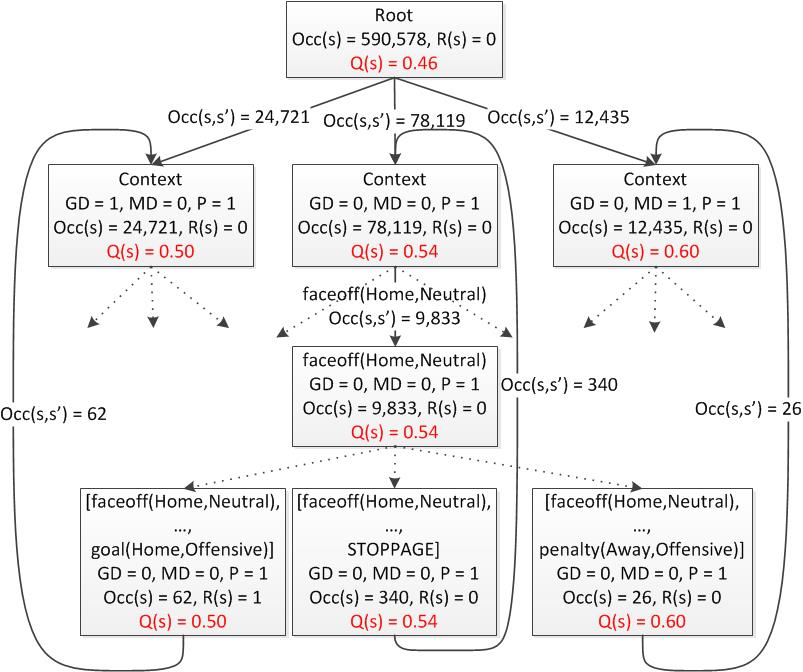
\includegraphics[width = 1.0\columnwidth]{sample_state_transition_graph2}
%\vspace{1in}
\caption{State Transition Graph}
\label{fig:state-transition-graph}
\end{figure}

Since the complete action history is encoded in the state, action-state pairs are equivalent to state pairs.
%Therefore we can model transitions from state to state only, rather than transitions from state to state given an action, even though we are mainly interested in the effects of actions.
For example, we can write $Q(\mstate \star \action)$ to denote the expected reward from taking action $\action$ in state $\mstate$, where $Q$ maps states to real numbers, rather than mapping action-state pairs to real numbers, as is more usual.
%In reinforcement learning terms, this means the $Q$-function can be computed by value iteration applied to states.

%A successor state $s' = s \star a_{n+1}$ represents the play sequence consisting of action events $a_1,a_2,\ldots,a_n,a_{n+1}$ and a particular $GD$, $MD$, and $P$.


%
%\begin{itemize}
%\item The action transition function $T$ is a 1-to-1 mapping of tuple $\mstates \times \actions \rightarrow \mstates$. In this restricted multi-agent environment, only one team can perform an action from each state, although not in a turn-based sequence. For example, if $a_{home}=$FACEOFF, then $a_{away}=$NO OPERATION, and $a_{home}$ is recorded as $a$.
%\end{itemize}
%
%An
%
%An \textbf{action} is therefore a pair (Team, Action-Event). An event history is a sequence of \textbf{events} with at most one start and end marker. A \textbf{state} contains the current context of the match, which includes the goal differential $GD$, manpower differential $MD$, and period $P$, as well as the event-history at the time of an action.

%, and the Markov Game Model contains $1,325,852$ nodes of states and events.

%%The following notation is used to describe the state space in NHL play sequences and player actions, and is used in the MDP construction and Value Iteration algorithms.
%MDP notation follows \citep{Russell2010}, and a modification of the notation used by \citep{Littman1994} is used to describe the multi-agent setup specific to NHL games. Notation for value iteration follows \citep{Mitchell1997}.





%\item We exclude zone from the context space, as it is not typically fixed throughout a play sequence, but include it as an attribute of player actions instead.
%{\em Make sure all notation is defined before you use it.} If in doubt, try to use fewer symbols and more English. Halmos has said that ``the best notation is no notation''. In a short conference paper, it's often a good idea to define all your symbols in this section. In a longer paper, it may be a good idea to define symbols close to where you use them.


%\subsection{EXAMPLES}

%Readers love examples, working through one to illustrate a definition is fine. For authors, they are a pain, because you already understand your concepts. Plus, it's easy to make small mistakes in an example, especially if you change it around. An ideal to aim for is to have a paper where the reader can read through examples, look through the figures and theorems, and get the idea of your paper without having to read through any details. Another reason to provide an example is this: suppose you guessed wrong about the level of background of  your reviewers, and failed to explain  a background concept so they could understand it. Or suppose you just forgot to define a concept. With an example, the reviewers can often recover from these gaps and get an idea of what you meant.

%\section{REWARDS}


%We use a computation for a Q-function in a policy-on setting, rather than a computation for a V-function typically used in reinforcement learning for computation following an optimal policy. %This is because our focus is on evaluating states and actions rather than determining an optimal policy.
%By calculating the difference in Q-values between two states, the impact of the corresponding action between the two states can be calculated.

%\section{VALUE ITERATION}

%\subsection{STATE TRANSITION GRAPH}


%[the informal description is good but should probably be merged with the more formal description. discuss AD-tree]

%\label{sec:algorithms}

%This should actually be relatively easy to write, since you are now focusing on your own work. It's often a good idea to start here, like two months before the submission deadline (see Poole above), and leave the trickier early parts for later. This is the part of the paper that is the hardest to read for referees, because it is about details and your new ideas rather than things they already know. So the challenge is to present your system in a way that's as simple and appealing as possible so a referee will be inclined to look at the details.

%\subsection{VALUE ITERATION}
%[explain value, how it is game-theoretic. Take perspective of single agent for MDP]



%Try to say in words what the key idea of your algorithm is.

%\subsection{PSEUDOCODE}


\subsection{REWARD FUNCTIONS: NEXT GOAL AND NEXT PENALTY}
\label{subsec:reward}

A strength of Markov Game modelling is value iteration can be applied to many reward functions depending on what results are of interest.
We focus on two: scoring the next goal, and receiving the next penalty (a cost rather than a reward).
These are two important events that change the course of an ice hockey game.
For example, penalties affect goal scoring differentials, as shown in Table~\ref{table:context-statistics}.
Penalties are also one path to goals that a coach may want to understand in more detail.
For instance, if a team receives an unusual number of penalties, a coach may want to know which players are responsible and by which actions.
%, and the corresponding Q-functions are easily interpreted.
%We have computed Q-functions for other reward functions but do not present these due to lack of space.
%Recall that states encode action histories. So we can define rewards as being associated with states only rather than state-action pairs.
The next goal objective can be represented in the Markov Game model as follows.



%This is to facilitate modelling different aspects of hockey dynamics.

%For the same reason, we can think of rewards as being associated with states only rather than state-action pairs. %

\begin{enumerate}
\item For any state $\mstate$ with a complete play sequence that ends in a Home resp. Away goal, we set $\reward_{\home}(\mstate) := 1$ resp. $\reward_{\away}(\mstate) := 1$. For other states the reward is 0.
\item Any state $\mstate$ with a complete play sequence that ends in a Home resp. Away goal is an absorbing state (no transitions from this state).
\end{enumerate}
%
%    \item $R_{\team}(s)$ is the reward value for each state $s$ received by team $\team$. This value depends on the objective being analyzed. $R_{\mstate} \equiv R_{\home}(\mstate)- R_{\away}(\mstate)$ is the reward differential, relative to the home team.
%\item Any $\mstate$ with a complete play sequence that ends in a Home resp. Away goal is an absorbing state (no transitions from this state).
%\item $Q_{\team}(\mstate)$ is the expected total reward obtained by a team, over all state sequences that start in state $\mstate$. $Q_{\mstate} \equiv Q_{\home}(\mstate)- Q_{\away}(\mstate)$ is \textbf{value} of state $\mstate$, relative to the home team.
%\item $Q_{i}(s)$ is the value iteration function value for state $s$ during iteration $i$. Note that $Q_{0}(s) = 0$ as an initialization step for the value iteration algorithm.


With these definitions, the expected reward %$Q_{\home}(\mstate)$
%
represents the probability that if play starts in state $\mstate$, a random walk through the state space of unbounded length ends with a goal for the Home team resp. the Away team. The cost function for Receiving the Next Penalty can be represented in exactly the same way.
%
%In a single-agent setting with a fixed policy, the value of a state is the expected reward for following the policy from the state. In the game-theoretic setting with two agents, we need to consider the difference in rewards. In a zero-sum game, the value of a state is the final result following optimal play. Intuitively, the value specifies which player has a better position in a state. Since we are not modelling optimal play, but actual play in a policy-on setting, the expected difference in rewards is the natural counterpart. We define the total reward over a state sequence as the sum of rewards, and while typically computed with a discount factor, discounting or averaging is not natural in ice hockey. For example, winning the game has the same value for a team regardless of how many actions occurred previously. Goals may be more valuable if they are scored after fewer actions, but this should be an empirical finding from the analysis, not built into the definition of the reward function. As such, we do not discount, following \citep{Schwartz1993}. Using undiscounted rewards raises issues about the convergence of an infinite sum of rewards. We discuss these below in connection with the value iteration algorithm.


\section{CONSTRUCTING THE STATE TRANSITION GRAPH}
\label{subsec:mdp-construction}

The main computational challenge is to build a data structure for managing the state space. The state space is large because each (sub)sequence of actions defines a new state. Since we are modelling the actual hockey dynamics in the ``on policy" setting, we need consider only action sequences observed in some NHL match, rather than the much larger space of all possible action sequences. We use the classic AD-tree structure \citep{Moore1998} to compute and store sufficient statistics over observed action sequences.
The AD-tree is a tree of play sequences where a node is expanded only with those successors observed in at least one match.
The play sequence tree is augmented with additional edges that model further state transitions; for example, a new action sequence is started after a goal.
The augmented AD-tree structure compactly manages sufficient statistics, in this case state transition probabilities.
It also supports value iteration updates very efficiently.


%Plays in the NHL form natural sequences of actions, typically starting with a faceoff and ending with a goal, penalty, or play stoppage. %These events can be viewed as a choice of actions by each team.
%It is intuitive to then transform these sequence of events into a game tree, where each subsequent event in a sequence is the child of the preceding event. We are also taking into account the context in which a play sequence occurs, so the tree must include the starting context of each play sequence as a state. The graph construction is performed as follows: the tree begins with a root state, or root node, where there is no context or sequence information. This is followed by the node representing the context of the game the play is starting in. Then the sequence of events follows below the context node, with branches forming as different events occur over multiple sequences. The process is repeated for each new play sequence by starting from the root node and adding new states, or nodes in the graph, as new action sequences are observed. Actions, such as penalties, often have an effect on the following sequences of actions. In order to propagate these effects, an edge is added from each leaf node of a play sequence, which represents a play sequence ending with a goal, penalty, or stoppage, to the context state node of the following play sequence. This transforms the graphical model from a tree into a multi-agent Markov Decision Process called a Markov Game Model. A sample of our Markov Game Model is shown in Figure~\ref{fig:state-transition-graph}. For an in-depth explanation of Markov Decision Processes, refer to \citep{Russell2010}. For more details on Markov Game Models, refer to \citep{Littman1994}.

We outline an algorithm for Context-Aware State Transition Graph construction. The root node initializes the graph, and is an empty node with no context or event information. For each node, the context information $GD$, $MD$, and $P$ are set when the new node is created, and the new action $a$ is added to the sequence along with the zone $Z$ that $a$ occurs in. The reward $R(s)$ is also applied to each node.
%, and the value of $R(s)$ is dependent on the objective function.
The node counts $Occ(s)$ and edge counts $Occ(s,s')$ are applied to each node and edge respectively, and are used to generate transition probabilities $TP$ for the value iteration using observed frequencies. %The function $incrementCount(s)$ is used to set node count $Occ(s)$, and $incrementCount(s,s')$ is used to set edge count $Occ(s,s')$.
The NHL play-by-play event data records goals, but no separate event for the shot leading to the goal exists. Following \citep{Schuckers2013}, we record the shot leading to the goal in addition to the goal itself by injecting a shot event into the event sequence prior to the goal.
%First, we create Next, we create a penalty state transition graph containing only loopback edges from penalty leaf nodes to propagate the effect of a penalty. Finally, the full state transition graph includes loopback edges from all leaf nodes.
%The sizes of these three graphs are shown in Table~\ref{table:size-of-graphs}.%A node denoting which team, home or away, won the match is added to the Markov Game Model after all events for the match have been processed into the graph.
%When values are backed up to the root node, the values are overall probabilities or expected values without any context information.
%[OS: probably better have example than pseudocode]
%\begin{algorithm}
%\caption{Context-Aware Markov Game Model Construction}
%\label{alg:mdp-construction}
%\begin{algorithmic}[1]
%    \REQUIRE NHL play-by-play data%, win data $w$
%    \STATE $root = new\ Node(empty)$
%    \FORALL{games $g$}
%        \STATE $current = root$
%        \STATE $previous = null$
%        \STATE $lastLeaf = false$
%        \FORALL{events $i$ in game $g$}
%            \IF{$current == root$}
%                \STATE{$incrementCount(root)$}
%                \STATE $state = i.getStateInformation$
%                \IF{not\ $root.hasChild(state)$}
%                    \STATE{$root.addChild(state)$}
%                \ENDIF
%                \STATE{$current = state$}
%                \STATE{$incrementCount(current)$}
%                \STATE{$incrementCount(root,current)$}
%                \IF{$lastLeaf == true$}
%                    \IF{not\ $previous.hasChild(current)$}
%                        \STATE{$previous.addChild(current)$}
%                    \ENDIF
%                    \STATE{$incrementCount(previous,current)$}
%                    \STATE{$lastLeaf = false$}
%                \ENDIF
%            \ENDIF
%            \IF{$i==$GOAL}
%                \STATE{$shotEvent = new\ Node(i,``SHOT")$}
%                \IF{not\ $current.hasChild(shotEvent)$}
%                    \STATE{$current.addChild(shotEvent)$}
%                \ENDIF
%                \STATE{$incrementCount(current,shotEvent)$}
%                \STATE{$incrementCount(shotEvent)$}
%                \STATE{$previous = current$}
%                \STATE{$current = shotEvent$}
%            \ENDIF
%            \STATE{$event = new\ Node(i)$}
%            \IF{not\ $current.hasChild(event)$}
%                \STATE{$current.addChild(event)$}
%            \ENDIF
%            \STATE{$incrementCount(current,event)$}
%            \STATE{$incrementCount(event)$}
%            \STATE{$previous = current$}
%            \STATE{$current = event$}
%            \IF{$current.isEndMarker()$}
%                \STATE{$lastLeaf = true$}
%                \STATE{$previous = current$}
%                \STATE{$current = root$}
%            \ENDIF
%        \ENDFOR
% %       \STATE{$win = new\ Node(w)$}
% %       \IF{not\ $previous.hasChild(win)$}
% %           \STATE{$previous.addChild(win)$}
% %       \ENDIF
% %       \STATE{$incrementCount(previous,win)$}
% %       \STATE{$incrementCount(win)$}
%    \ENDFOR
%\end{algorithmic}
%\end{algorithm}

%\begin{table}[htb]
%\caption{Size of State Transition Graphs}
%\label{table:size-of-graphs}
%\begin{center}
%\resizebox{\columnwidth}{!}{
%\begin{tabular}{|l|c|c|c|}
%\hline
%& \bf{Local} & \bf{Penalty} & \bf{Full} \\ \hline
%\bf{Number of Nodes} & 1,325,809 & 1,325,809 & 1,325,809 \\ \hline
%\bf{Number of Edges} & 1,325,808 & 1,382,780 & 1,662,504 \\ \hline
%\end{tabular}
%}
%\end{center}
%\end{table}



\section{VALUE ITERATION}
\label{subsec:value-iteration-alg}

Recall that since states encode action histories, in our model learning the expected value of states is equivalent to learning a Q-function (Section~\ref{subsec:transitions}). In reinforcement learning terms, there is no difference between the value function V and the Q-function in our model. We can therefore apply standard value iteration over states \citep{bib:sutton} to learn a Q-function
 for our ice hockey Markov Game. Algorithm~\ref{alg:value-iteration-dynamic} shows pseudo-code. We compute separate Q-functions for the Home team and for the Away team. Since we are in the ``on policy" setting, we have a fixed policy for the other team. This means we can treat the other team as part of the environment, and reduce the Markov Game to two single-agent Markov decision processes. % for the purpose of value iteration.
 In our experiments, we use a relative convergence of 0.0001 as our convergence criterion, and 100,000 as the maximum number of steps.% Value iteration converges in at most 10,050 iterations in all our experiments.
%
%
%For the probability of the next goal, or next penalty, Equation~\ref{equation:value-iteration-probability} is used as the value iteration function. Here, $a$ can be goal or penalty, and $T$ can be Home or Away. For example, if you want to find the probability of the next home goal, then $a$ would be goal, $T$ would be home, and $a(T,*)$ would be a home goal scored from any zone. All events matching $a(*,*)$ are excluded from the first summation in Equation~\ref{equation:value-iteration-probability}. This facilitates backing up the value $0$ for the opposite $T$. For example, if $a$ is goal and $T$ is Home, goal(Away,*) is excluded from the summation, equivalent to backing up $0$ for goal(Away,*).
%
%
%
%Now that the Markov Game Model for the play-by-play events has been generated, the next step is to run a dynamic programming algorithm for value iteration to extract the values of different actions in different states. As the game is zero-sum, the value iteration will give expected rewards or the probability of rewards for each action, which can be applied to a single agent taking the action. The computation can be performed over many objective functions simultaneously, and is run iteratively until a convergence criterion is met or a maximum number of iterations is reached. For our experiments, we used six objective functions shown in Table~\ref{table:value-iteration-computation}. Conditional Probabilities for goal scoring and receiving a penalty can also be derived by combining the probabilistic objectives for the home team and away team. These node values are then used to compute action values specific to each node, as the action values are dependent on the context and event history. As players perform these actions in a match, the action values are applied to the players and are used to evaluate player performance. For an in-depth explanation of value iteration for reinforcement learning, refer to \citep{Mitchell1997}. We use an undiscounted Q-function for our value iteration, following \citep{Schwartz1993}.
%
%\begin{table}[htb]
%\caption{Reward Functions}
%\label{table:value-iteration-computation}
%\begin{center}
%\resizebox{1\columnwidth}{!}{
%\begin{tabular}{|l|}
%\hline
%%Expected Wins \\ \hline
%%Probability of the Home Team Winning \\ \hline
%%Probability of the Away Team Winning \\ \hline
%Expected Goals \\ \hline
%Probability that the Home Team Scores the Next Goal \\ \hline
%Probability that the Away Team Scores the Next Goal \\ \hline
%Expected Penalties \\ \hline
%Probability that the Home Team Receives the Next Penalty \\ \hline
%Probability that the Away Team Receives the Next Penalty \\ \hline
%\end{tabular}
%}
%\end{center}
%\end{table}
%
%For expected values of goals or penalties, Equation~\ref{equation:value-iteration-expected} is used as the Q-function. $R(s)$ is initialized based on the event being analyzed as an objective. For example, if the objective is to find the expected goals, $R(s) = 1$ when $s$ is a goal(Home,*), $R(s) = -1$ when $s$ is a goal(Away,*), and $R(s) = 0$ for all other events and states. This is done similarly for using penalties as the objective. Note that $\cfrac{Occ(s,s')}{Occ(s)}$ forms the transition probability from state $s$ to state $s'$, but $\cfrac{1}{Occ(s)}$ is factored out to the front of the summation to improve computation time.
%
%For the probability of the next goal, or next penalty, Equation~\ref{equation:value-iteration-probability} is used as the value iteration function. Here, $a$ can be goal or penalty, and $T$ can be Home or Away. For example, if you want to find the probability of the next home goal, then $a$ would be goal, $T$ would be home, and $a(T,*)$ would be a home goal scored from any zone. All events matching $a(*,*)$ are excluded from the first summation in Equation~\ref{equation:value-iteration-probability}. This facilitates backing up the value $0$ for the opposite $T$. For example, if $a$ is goal and $T$ is Home, goal(Away,*) is excluded from the summation, equivalent to backing up $0$ for goal(Away,*).

%The probability of the home team or away team winning is similar to Equation~\ref{equation:value-iteration-probability} but also includes the reward $R(s)=1$ for the EVENT being analyzed and $R(s)=0$ for all other states. This calculation is outlined in Equation~\ref{equation:value-iteration-probability-winning}.

%Once the objective functions are defined, the Value Iteration Dynamic Programming Algorithm can be executed on the MDP to determine the values of each state. The steps are outlined in Algorithm~\ref{alg:value-iteration-dynamic}. Algorithm~\ref{alg:value-iteration-dynamic} shows the algorithm with the Expected Goals or Expected Penalties computation shown in Equation~\ref{equation:value-iteration-expected}. To calculate other objectives, the calculation for $Q_{i+1}(s)$ can be replaced with Equation~\ref{equation:value-iteration-probability}.% or Equation~\ref{equation:value-iteration-probability-winning}.
%
%\begin{equation}
%\label{equation:value-iteration-expected}
%Q_{i+1}(s) = R(s) + \cfrac{1}{Occ(s)}\sum_{\substack{(s,s') \in E}}(Occ(s,s')\times Q_{i}(s'))
%\end{equation}
%
%\begin{multline}
%\label{equation:value-iteration-probability}
%Q_{i+1}(s) = \\
%\cfrac{1}{Occ(s)}(\big(\sum_{\substack{(s,s') \in E \\ s' \neq a(*,*)}}\Big(Occ(s,s') \times Q_{i}(s')\Big)\big) \\
%+ \big(\sum_{\substack{(s,s') \in E \\ s' = a(T,*)}}\Big(Occ(s,s') \times 1\Big)\big))
%\end{multline}

%\begin{multline}
%\label{equation:value-iteration-probability-winning}
%Q_{i+1}(s) = \\
%R(s) + \cfrac{1}{Occ(s)}(
%\big(\sum_{\substack{(s,s') \in E \\ s' \neq EVENT}}\Big(Occ(s,s')\times Q_{i}(s')\Big)\big) \\
%+ \big(\sum_{\substack{(s,s') \in E \\ s' = TEAM:EVENT}}\Big(Occ(s,s') \times 1\Big)\big))
%\end{multline}

\begin{algorithm}
\caption{Dynamic Programming for Value Iteration}
\label{alg:value-iteration-dynamic}
\begin{algorithmic}[1]
\REQUIRE Markov Game model, convergence criterion $c$, maximum number of iterations $M$
\STATE{$lastValue = 0$}
\STATE{$currentValue = 0$}
\STATE{$converged = false$}
\FOR{$i = 1; i \leq M; i \gets i + 1$}
    \FORALL{states $s$ in the Markov Game model}
        \IF{$converged == false$}
            \STATE{$Q_{i+1}(s) = $\\$R(s) + \cfrac{1}{Occ(s)}\sum_{\substack{(s,s') \in E}}(Occ(s,s')\times Q_{i}(s'))$}
            \STATE{$currentValue = currentValue + |Q_{i+1}(s)|$}
        \ENDIF
    \ENDFOR
    \IF{$converged == false$}
        \IF{$\frac{currentValue - lastValue}{currentValue} < c$}
            \STATE{$converged = true$}
        \ENDIF
    \ENDIF
    \STATE{$lastValue = currentValue$}
    \STATE{$currentValue = 0$}
\ENDFOR
\end{algorithmic}
\end{algorithm}

%Make sure all notation is defined.

%\subsection{CONVERGENCE} %Discuss convergence.
%
%Each iteration $i$ of the dynamic programming algorithm computes the value of a state with a lookahead window of at most $i$ steps. As the limit of $i$ goes to infinity, each path of at most $i$ steps from a state will either end in the objective event, such as a goal, or the end of the match. The occurrences of the end of match are much smaller than the number of goals or penalties, so approximately every path will end with the objective event for either the home team or the away team. As such, the value of each state will converge to the conditional probability of the home or away team's objective event. As we use rewards with bounded sums, the computations of expected values also converge by extension.

%\subsection{EXAMPLE}
%
%We will first give a small example of the context-inclusive Markov Decision Process construction. This will be followed by a few iterations of the value iteration dynamic programming algorithm.


%Readers love examples, stepping through a computation is fine.

%\subsection{THEORETICAL JUSTIFICATION}

%Sometimes this comes first, for instance if your algorithm is based on a mathematical derivation. You could also at this point include a correctness proof, or a complexity analysis (e.g., theoretical upper bound on run-time).

%\subsection{DISCUSSION}

%The context state space consists of goal differential, manpower differential, and period as context variables. Goal differential, manpower differential, and period typically remain fixed during a play sequence. The exception to this rule is that manpower differential can change during a play sequence when the goalie is pulled or a penalized player returns to the ice. The zone was left out context state space in order to decrease the number of context subtrees, which also reduces the number of nodes. Instead, zone is included in the action-event. %The change in the number of states with and without manpower differential is observed in Table~\ref{table:size-of-mdp}.

%There may be a need for discussion, for instance why you made certain design choices or how your algorithm is different from that used by others.

%\section{SYSTEM, EVALUATION AND RESULTS}
\section{EVALUATION AND RESULTS}

%The hardware used in our data collection, model construction, and value iteration computation are summarized in Section~\ref{sec:hardware}.
We discuss the results of action values in Section~\ref{subsec:action-values} and player values in Section~\ref{subsec:player-valuations}. Our state transition graph is evaluated in Section~\ref{subsec:lesion-study}.

%For evaluating our method, we first examine the information from the play-by-play data by examining the context contingency table without including sequence history. Next, we discuss the benefit of including cross-sequence loops in the Markov Game Model. We then use the Markov Game Model with cross-sequence loops to determine the values of each action, and compare with action values computed in previous works. Finally, we use our action values derived from the value iteration computation to score and rank NHL players, and compare player scores with salaries.

%\subsection{SYSTEM}
%\label{sec:hardware}
%
%NHL play-by-play data was obtained from \url{http://www.nhl.com} using the Selenium WebDriver with Python 2.7.6. Markov Game Model construction and value iteration computation was performed using Java Version 8 Update 25 on 64-bit Windows 7 with 12GB RAM and an Intel Core i7-2670QM CPU @ 2.20GHz $\times$ 8. The state transition graph is stored in a MySQL 5.6.13 database.
% using two tables for nodes and edges.

%This is another important section for referees. Part of the attraction is that they can look at your performance numbers and your methodology and criticize it without having understood the details of your method. Unfortunately, most parts of computer science don't have a fixed evaluation methodology. It is therefore hard to anticipate what reviewers will consider critical. So if in doubt, do more: report more measurements, do more statistical significance tests, try more datasets, try more parameter settings for the methods, look at different sample sizes, etc. I realize that running more experiments can be a lot of work, so students are often tempted to try and do the minimum necessary for acceptance. It's just that nobody knows what that minimum is. Sometimes it's a good idea to send the paper to a workshop, to get some feedback on the evaluation.

%Running a set of experiments is likely the most complex programming project you have ever done. It will pay to try and follow a good practice so you don't have to relearn tricks the hard way (i.e., always save your output files). The following website presents some nice advice from someone who has been there: http://arkitus.com/PRML/.

%\begin{figure}[ht]
%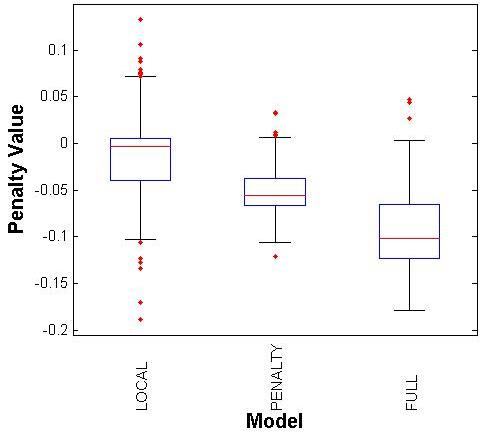
\includegraphics[width = 1.0\columnwidth]{penalty_value_vs_graph}
%%\vspace{1in}
%\caption{Change In Value Of Penalty For Goals}
%\label{fig:boxplot-penalty-values}
%\end{figure}

%All artwork must be centered, neat, clean, and legible. Figure number
%and caption always appear below the figure.  Leave 2 line spaces
%between the figure and the caption. The figure caption is initial caps
%and each figure numbered consecutively.
%
%Make sure that the figure caption does not get separated from the
%figure. Leave extra white space at the bottom of the page rather than
%splitting the figure and figure caption.

%[OS: use box plots]
%
%\begin{table}[htb]
%\caption{Lock and Schucker's Action Values (Previous Values) vs. Value Iteration Action Values}
%\label{table:action-values}
%\begin{center}
%\resizebox{1\columnwidth}{!}{
%\begin{tabular}{|c|c|c|c|c|c|}
%\hline
%\bf{Action} & \bf{Previous Value} & \multicolumn{4}{|c|}{\bf{Value Iteration}} \\ \cline{3-6}
% & & Weighted Average & Maximum & Minimum & Variance \\ \hline
%Blocked Shot & 0.0957 & 0.0004 & 0.5025 & -0.5785 & 0.0004 \\ \hline
%Faceoff (Defensive) & -0.0017 & & & & \\ \hline
%Faceoff (Neutral) & 0.0007 & & & & \\ \hline
%Faceoff (Offensive) & 0.0110 & & & & \\ \hline
%Giveaway & -0.0226 & -0.0020 & 0.5609 & -0.6065 & 0.0006 \\ \hline
%Hit & -0.0046 & -0.0001 & 0.6057 & -0.5208 & 0.0003 \\ \hline
%Missed Shot & 0.0094 & -0.0004 & 0.5890 & -0.6009 & \\ \hline
%Penalty & -0.1534 & -0.0072 & 0.1364 & -0.1920 & \\ \hline
%Shot & 0.1226 & 0.0063 & 0.5804 & -0.5008 & \\ \hline
%Takeaway & 0.0174 & 0.0018 & 0.5530 & -0.5763 & \\ \hline
%\end{tabular}
%}
%\end{center}
%\end{table}

\subsection{ACTION IMPACT VALUES}
\label{subsec:action-values}

The main quantity we consider is the \textbf{impact} of an action as a function of context (= Markov state). This is defined as follows:

\begin{equation*}
\impact(\mstate,\action) \equiv Q_{\team}(\mstate \star \action) - Q_{\team}(\mstate)
\end{equation*}
%\begin{itemize}
%\item The \textbf{value} of a state is the difference in expected rewards: $Q_{\mstate} \equiv Q_{\home}(\mstate)- Q_{\away}(\mstate)$.
%\item For a state $\mstate$ with an incomplete play sequence, the quantity $\impact(\action) \equiv Q(\mstate \star \action) - Q(\mstate)$ is the \textbf{impact} of the action $\action$ on the value of the state.
%\end{itemize}
where $\team$ is the team executing the action $\action$. In a zero-sum game, the state value is usually defined as the final result following optimal play \citep{Russell2010}. Intuitively, the value specifies which player has a better position in a state. Since we are not modelling optimal play, but actual play in an ``on policy" setting, the expected difference in rewards is the natural counterpart. The impact quantity measures how performing an action in a state affects the expected reward difference.
Figure~\ref{fig:boxplot-action-values} shows a boxplot for the action impact values as they range over different contexts, i.e., states in the Markov Game model.
% defined with scoring the next goal as the reward
(Boxplots produced with MATLAB R2014a.)
The central mark is the median, and the edges of the boxes are the 25th and 75th percentiles.
The whiskers are the default value, approximately 2.7 standard deviations.
The red dots are outliers beyond 2.7 s.d. and the asterisks are the values given for each action in \citep{Lock2009}.
A cutoff of -0.2 and 0.2, represented by the horizontal dashed line, was used for the impact values on both boxplots.
% Probability of the Next Home Goal as the objective function.
% Positive values are in favor of the a player's team, and negative values are in favor of their opponent.
While the Q-values are based on the frequency of states, we weight all states equally in discussing the properties of the Q-function. The boxplot does not include Q-values for states whose frequency is below 5\%.
It is clear from Figure~\ref{fig:boxplot-action-values} that {\em depending on the context and event history, the value of an action can vary greatly.} The context-dependence is observed for both scoring goals and receiving penalties.

\paragraph{Impact on Scoring the Next Goal.} All actions, with the exception of faceoffs won in the offensive zone, have at least one state where the action has a positive impact, and another state with a negative impact. Specific examples of context-dependence that can be found by examining states with extreme impact values include the following.

 (1) After blocking the first shot on net when killing a penalty, the shooting team tends to score more goals $(impact=-0.0864)$. But after blocking the second shot on net, the blocking team tends to score more goals $(impact=0.1399)$.

 (2) Receiving a penalty when on the powerplay is very bad $(impact=-0.1789)$, but if a player on the penalty kill can goad their opponent into an offsetting penalty, it is good $(impact=0.0474)$.

The THoR player ratings compute the impact of actions based on goals that immediately follow the action (\citep{Lock2009,Schuckers2011}; see Section~\ref{sec:related-work}).
The values given for each action in \citep{Lock2009} are displayed as an asterisk in Figure~\ref{fig:goal-impact}.
%
%We compare the impact values computed for each action from our value iteration algorithm with the fixed values computed in \citep{Lock2009,Schuckers2011}. The values computed for each action in \citep{Lock2009} are displayed as an asterisk in Figure~\ref{fig:boxplot-action-values}.
% should compare by averaging over all states.
 %
The THoR values
%\citep{Lock2009}
agree with our median impact values in terms of whether an action generally has positive or negative impact. For example, penalties are known to generally be good for the opposing team, and shots are good for the shooter's team. THoR values are close to the median Markov model values in 6 out of 10 cases.
%The exceptions are blocked shots, faceoffs won in the offensive zone, penalties, and shots.
This comparison suggests that THoR aggregates action values over many contexts that the Markov game models explicitly.
%, but the postive/negative team bias found in \citep{Lock2009} for each agrees with our medians.
%For example, penalties are known to generally be good for the opposing team, and shots are good for the player's team.
% The most notable change in action value was observed in the value of a penalty, shown in Figure~\ref{fig:boxplot-penalty-values}.



\paragraph{Impact on Receiving Penalties.}
The range of action values with the probability of the next penalty as the objective function is shown in Figure~\ref{fig:penalty-impact}.
%Again we observe that the impact of actions on penalties varies greatly with context.
Faceoffs in the Offensive Zone and takeaways cause penalties for the opponent. Giveaways and goals tend to be followed by a penalty for the player's team. This finding is consistent with the observation that there are fewer penalties for teams with higher leads \citep{Schuckers2012}. A possible explanation is referees are reluctant to penalize a trailing team.
%are most likely to cause that team to receive the next penalty.

\begin{figure*}[ht]
\centering
\hbox{
\subfigure[Impact on the probability of Scoring the Next Goal. Higher numbers are {\em better} for the team that performs the action.]{
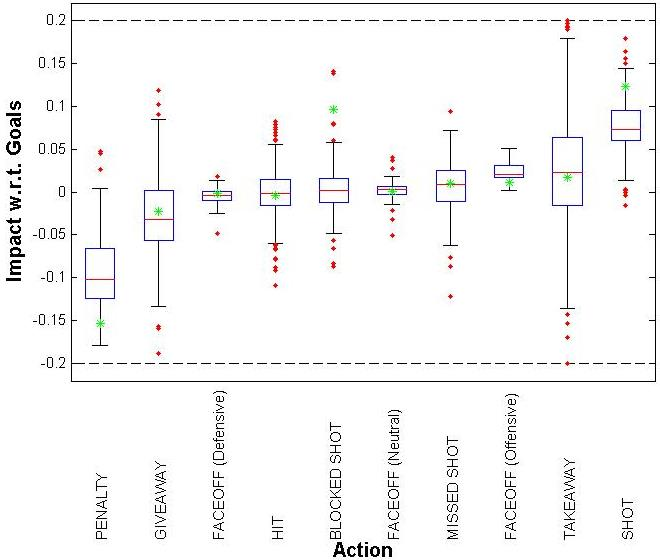
\includegraphics[width = 1.0\columnwidth]{action_values_full_probability_next_goal_w_lock}
%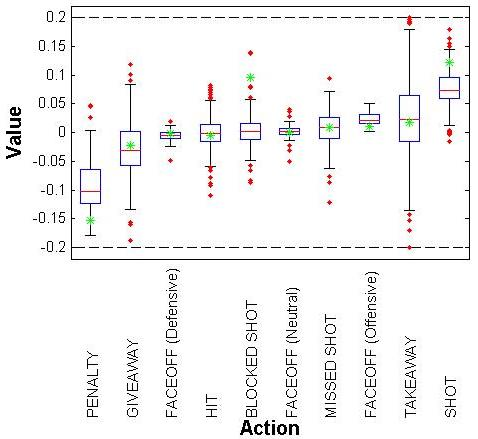
\includegraphics[width = 1.0\columnwidth]{boxplot_actionvalues4}
%\vspace{1in}
\label{fig:goal-impact}
}
\subfigure[Impact on the probability of Receiving the Next Penalty. Higher numbers are {\em worse} for the team that performs the action.]{
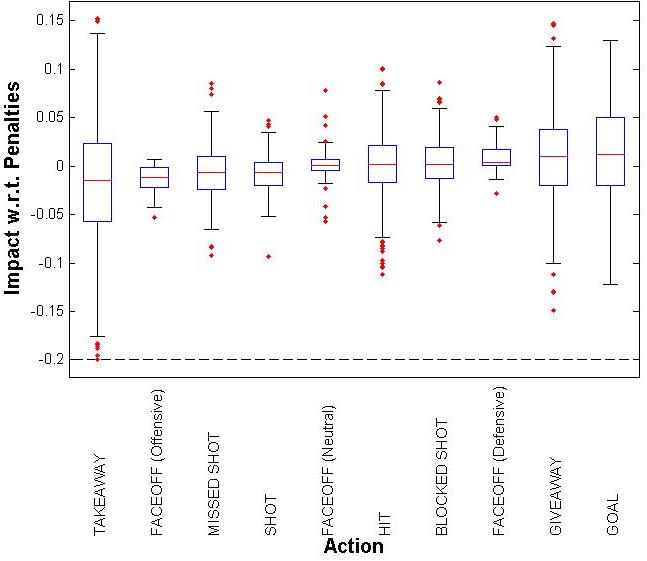
\includegraphics[width = 1.0\columnwidth]{action_values_full_probability_next_penalty}
%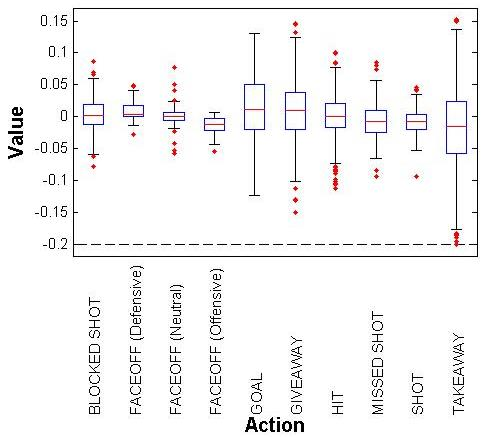
\includegraphics[width = 1.0\columnwidth]{boxplot_penalty_value_full}
%\vspace{1in}
%\caption{Action Value Ranges For Penalties}
%\label{fig:boxplot-action-values-penalties}
\label{fig:penalty-impact}}}

\caption{Action Impact Values vary with context. The central mark is the median, the edges of the box are the 25th and 75th percentiles. The whiskers are at the default value, approximately 2.7 s.d.}
\label{fig:boxplot-action-values}
\end{figure*}

%
%\begin{figure}[ht]
%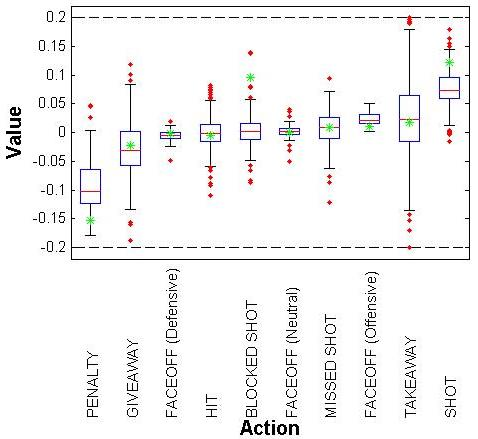
\includegraphics[width = 1.0\columnwidth]{boxplot_actionvalues4}
%%\vspace{1in}
%\caption{Action Impact Values For Goals. The central mark is the median, the edges of the box are the 25th and 75th percentiles. The whiskers are the default value, approximately 2.7 sd.}
%\label{fig:boxplot-action-values}
%\end{figure}
%
%\begin{figure}[ht]
%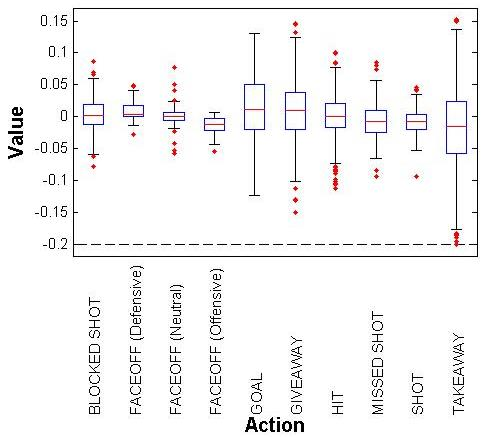
\includegraphics[width = 1.0\columnwidth]{boxplot_penalty_value_full}
%%\vspace{1in}
%\caption{Action Value Ranges For Penalties}
%\label{fig:boxplot-action-values-penalties}
%\end{figure}

\begin{figure}[ht]
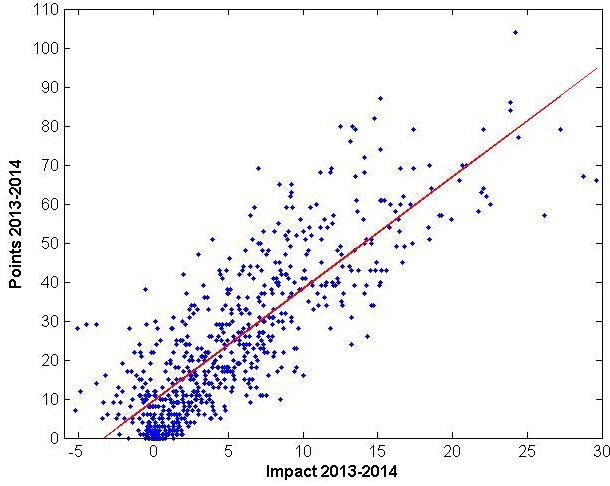
\includegraphics[width = 1.0\columnwidth]{points_vs_impact}
%\vspace{1in}
\caption{2013-2014 Player Goal Impact Vs. Season Points}
\label{fig:points-vs-impact}
\end{figure}



%\subsection{State Statistics and Values: No Sequences}
%
%general strategy: winning chance changes with goal scoring (goal diff). Goal scoring changes with penalties.  Dtree can tell you how to achieve goals or penalities locally. State backup integrates these numbers into a single one, for both goal scoring and penalty achievement. (Player ranking?)

%\begin{table*}[htb]
%\caption{Play-by-Play Sequence Contingency Table}
%\label{table:contingency-table}
%\begin{center}
%\resizebox{1\textwidth}{!}{
%\begin{tabular}{|c|c|c|c|c|c|c|c|c|}
%\hline
% \bf{Goal Differential} & \bf{Manpower Differential} & \bf{Period} & \bf{Number of Sequences} & \bf{Ends In Goal} & \bf{Ends In Penalty} & \bf{Reward = Win} & \bf{Reward = Goal} & \bf{Reward = Next Home Goal} \\ \hline
%0 & 0 & 1 & 69,358 & 4,924 & 10,014 & -0.000013206 & 0.003394622 & 0.017470455 \\ \hline
%0 & 0 & 2 & 33,976 & 2,602 & 5,233 & 0.000006222 & 0.003367201 & 0.021706954 \\ \hline
%0 & 0 & 3 & 26,741 & 1,821 & 2,787 & -0.000206337 & 0.002227779 & 0.019534592 \\ \hline
%1 & 0 & 2 & 26,482 & 2,097 & 4,221 & 0.000380054 & 0.001543053 & 0.021591389 \\ \hline
%1 & 0 & 3 & 22,826 & 1,831 & 2,666 & 0.044373381 & 0.002387631 & 0.024226838 \\ \hline
%-1 & 0 & 2 & 22,566 & 1,760 & 3,538 & -0.000382451 & 0.003115098 & 0.022845692 \\ \hline
%1 & 0 & 1 & 22,066 & 1,480 & 3,568 & 0.000000085 & 0.003423563 & 0.019661919 \\ \hline
%-1 & 0 & 3 & 19,964 & 1,565 & 2,276 & -0.046039697 & 0.001331026 & 0.021621996 \\ \hline
%-1 & 0 & 1 & 18,495 & 1,305 & 2,948 & -0.000000221 & 0.004565380 & 0.020117038 \\ \hline
%2 & 0 & 3 & 15,585 & 1,297 & 2,027 & 0.066432887 & 0.004187012 & 0.026217242 \\ \hline
%2 & 0 & 2 & 13,763 & 1,081 & 2,338 & 0.000709842 & 0.001615879 & 0.023955375 \\ \hline
%-2 & 0 & 3 & 12,314 & 962 & 1,489 & -0.071100171 & -0.001731899 & 0.023280575 \\ \hline
%-2 & 0 & 2 & 10,497 & 794 & 1,691 & -0.000812391 & 0.004713458 & 0.022603555 \\ \hline
%0 & 1 & 1 & 10,265 & 1,260 & 1,650 & -0.000000238 & 0.068621551 & 0.040057357 \\ \hline
%0 & -1 & 1 & 9,689 & 1,055 & 1,819 & -0.000000263 & -0.056201080 & 0.015560972 \\ \hline
%3 & 0 & 3 & 9,557 & 597 & 1,626 & 0.095149511 & -0.001446753 & 0.02112544 \\ \hline
%-3 & 0 & 3 & 6,715 & 410 & 1,060 & -0.100993803 & 0.003415244 & 0.021614998 \\ \hline
%0 & 0 & 4 & 6,252 & 640 & 474 & 0.000267494 & 0.005802195 & 0.034859076 \\ \hline
%0 & 1 & 2 & 6,150 & 723 & 955 & -0.000000770 & 0.058506601 & 0.043446392 \\ \hline
%3 & 0 & 2 & 5,684 & 423 & 1,051 & 0.000901368 & -0.002641091 & 0.023404221 \\ \hline
%0 & -1 & 2 & 5,679 & 672 & 970 & 0.000191954 & -0.057690825 & 0.019719806 \\ \hline
%2 & 0 & 1 & 5,347 & 345 & 931 & 0.000000315 & 0.002314936 & 0.019898360 \\ \hline
%1 & -1 & 2 & 4,836 & 606 & 753 & 0.000224084 & -0.063834184 & 0.020434313 \\ \hline
%1 & 1 & 2 & 4,682 & 579 & 805 & 0.000329883 & 0.063028993 & 0.047728124 \\ \hline
%\end{tabular}
%}
%\end{center}
%\end{table*}

%\begin{table*}[htb]
%\caption{Period Four Play-by-Play Sequence Contingency Table. Goals are more common than penalties. Penalties are more favorable for the home team.}
%\label{table:period-four-ct}
%\begin{center}
%\resizebox{1\textwidth}{!}{
%\begin{tabular}{|c|c|c|c|c|c|c|c|c|}
%\hline
% \bf{Goal Differential} & \bf{Manpower Differential} & \bf{Period} & \bf{Number of Sequences} & \bf{Ends In Goal} & \bf{Ends In Penalty} & \bf{Reward = Win} & \bf{Reward = Goal} & \bf{Reward = Next Goal} \\ \hline
% 0 & 0 & 4 & 6,252 & 640 & 474 & 0.000267494 & 0.005802195 & 0.034859076 \\ \hline
%0 & 1 & 4 & 668 & 109 & 53 & 0.004224813 & 0.131447067 & 0.097894388 \\ \hline
%0 & -1 & 4 & 564 & 87 & 54 & -0.001124987 & -0.107908279 & 0.014118699 \\ \hline
%0 & -2 & 4 & 25 & 0 & 5 & 0.000070744 & 0.001409694 & 0.014042549 \\ \hline
%0 & 2 & 4 & 23 & 2 & 1 & 0.000109450 & 0.085741439 & 0.107596947 \\ \hline
%\end{tabular}
%}
%\end{center}
%\end{table*}

%\begin{table*}[ht]
%\caption{Statistics for Top-20 Context States}
%\label{table:context-statistics}
%\begin{center}
%\resizebox{1\textwidth}{!}{
%\begin{tabular}{|c|c|c|c|c|c|c|c|c|}
%\hline
%\bf{Goal Differential} & \bf{Manpower Differential} & \bf{Period} & \bf{Number of Sequences} & \bf{Winning Difference} & \bf{Number of Goals} & \bf{Goal Difference} & \bf{Number of Penalties} & \bf{Penalty Difference} \\ \hline
%0 & 0 & 1 & 78,118 & 9.7\% & 5,524 & 7.1\% & 11,398 & -2.3\% \\ \hline
%0 & 0 & 2 & 38,315 & 7.6\% & 2,935 & 7.6\% & 5,968 & -2.9\% \\ \hline
%0 & 0 & 3 & 30,142 & 2.9\% & 2,050 & 5.9\% & 3,149 & -2.2\% \\ \hline
%1 & 0 & 2 & 29,662 & 45.1\% & 2,329 & 2.0\% & 4,749 & 2.2\% \\ \hline
%1 & 0 & 3 & 25,780 & 60.6\% & 2,076 & 4.3\% & 3,025 & 3.5\% \\ \hline
%-1 & 0 & 2 & 25,498 & -33.2\% & 1,970 & 8.6\% & 4,044 & -8.7\% \\ \hline
%1 & 0 & 1 & 24,721 & 41.5\% & 1,656 & 5.3\% & 4,061 & 3.4\% \\ \hline
%-1 & 0 & 3 & 22,535 & -54.5\% & 1,751 & 0.7\% & 2,565 & -18.3\% \\ \hline
%-1 & 0 & 1 & 20,813 & -26.1\% & 1,444 & 4.6\% & 3,352 & -8.1\% \\ \hline
%2 & 0 & 3 & 17,551 & 88.4\% & 1,459 & 6.9\% & 2,286 & -0.9\% \\ \hline
%2 & 0 & 2 & 15,419 & 72.9\% & 1,217 & 2.7\% & 2,620 & 2.9\% \\ \hline
%-2 & 0 & 3 & 13,834 & -86.8\% & 1,077 & -2.3\% & 1,686 & -12.6\% \\ \hline
%0 & 1 & 1 & 12,435 & 11.9\% & 1,442 & 64.8\% & 2,006 & 65.9\% \\ \hline
%-2 & 0 & 2 & 11,799 & -68.0\% & 882 & 3.9\% & 1,927 & -15.7\% \\ \hline
%0 & -1 & 1 & 11,717 & 5.1\% & 1,260 & -54.8\% & 2,177 & -44.7\% \\ \hline
%3 & 0 & 3 & 10,819 & 97.2\% & 678 & 0.3\% & 1,859 & 1.2\% \\ \hline
%-3 & 0 & 3 & 7,569 & -94.2\% & 469 & 7.0\% & 1,184 & -6.3\% \\ \hline
%0 & 1 & 2 & 7,480 & 8.5\% & 851 & 57.0\% & 1,157 & 25.7\% \\ \hline
%0 & 0 & 4 & 7,024 & -0.6\% & 721 & 5.7\% & 535 & -10.7\% \\ \hline
%0 & -1 & 2 & 6,853 & 0.3\% & 791 & -52.5\% & 1,160 & -37.4\% \\ \hline
%\end{tabular}
%}
%\end{center}
%\end{table*}

%\begin{table*}[htbp]
%\caption{State Goal and Penalty Conditional Probability Table}
%\label{table:state-probabilities}
%\begin{center}
%\resizebox{1\textwidth}{!}{
%\begin{tabular}{|c|c|c|c|c|c|c|c|c|}
%\hline
% \bf{Goal Differential} & \bf{Manpower Differential} & \bf{Period} & \bf{Number of Sequences} & \bf{Probability of Home Goal} & \bf{Probability of Away Goal} & \bf{Probability of Home Penalty} & \bf{Probability of Away Penalty} \\ \hline
%0 & 0 & 1 & 69,358 & 53.43217 & 46.56783 & 49.10126 & 50.89874 \\ \hline
%0 & 0 & 2 & 33,976 & 53.99693 & 46.00307 & 48.86298 & 51.13702 \\ \hline
%0 & 0 & 3 & 26,741 & 52.60846 & 47.39154 & 48.83387 & 51.16613 \\ \hline
%1 & 0 & 2 & 26,482 & 51.40677 & 48.59323 & 51.07794 & 48.92206 \\ \hline
%1 & 0 & 3 & 22,826 & 52.70344 & 47.29656 & 51.91298 & 48.08702 \\ \hline
%-1 & 0 & 2 & 22,566 & 53.97727 & 46.02273 & 46.07123 & 53.92877 \\ \hline
%1 & 0 & 1 & 22,066 & 52.36486 & 47.63514 & 51.76570 & 48.23430 \\ \hline
%-1 & 0 & 3 & 19,964 & 50.60703 & 49.39297 & 40.64148 & 59.35852 \\ \hline
%-1 & 0 & 1 & 18,495 & 52.87356 & 47.12644 & 46.40434 & 53.59566 \\ \hline
%2 & 0 & 3 & 15,585 & 53.12259 & 46.87741 & 49.72866 & 50.27134 \\ \hline
%2 & 0 & 2 & 13,763 & 50.78631 & 49.21369 & 51.83918 & 48.16082 \\ \hline
%-2 & 0 & 3 & 12,314 & 49.58420 & 50.41580 & 43.45198 & 56.54802 \\ \hline
%-2 & 0 & 2 & 10,497 & 51.13350 & 48.86650 & 42.16440 & 57.83560 \\ \hline
%0 & 1 & 1 & 10,265 & 83.73016 & 16.26984 & 67.15152 & 32.84848 \\ \hline
%0 & -1 & 1 & 9,689 & 20.56872 & 79.43128 & 25.34360 & 74.65640 \\ \hline
%3 & 0 & 3 & 9,557 & 51.08878 & 48.91122 & 50.92251 & 49.07749 \\ \hline
%-3 & 0 & 3 & 6,715 & 53.65854 & 46.34146 & 46.69811 & 53.30189 \\ \hline
%0 & 0 & 4 & 6,252 & 52.18750 & 47.81250 & 44.72574 & 55.27426 \\ \hline
%0 & 1 & 2 & 6,150 & 79.39142 & 20.60858 & 63.66492 & 36.33508 \\ \hline
%3 & 0 & 2 & 5,684 & 50.59102 & 49.40898 & 53.47288 & 46.52712 \\ \hline
%0 & -1 & 2 & 5,679 & 22.17262 & 77.82738 & 30.82474 & 69.17526 \\ \hline
%2 & 0 & 1 & 5,347 & 52.46377 & 47.53623 & 54.45757 & 45.54243 \\ \hline
%1 & -1 & 2 & 4,836 & 21.12211 & 78.87789 & 35.72377 & 64.27623 \\ \hline
%1 & 1 & 2 & 4,682 & 81.17444 & 18.82556 & 65.21739 & 34.78261 \\ \hline
%\end{tabular}
%}
%\end{center}
%\end{table*}

%\begin{table*}[htb]
%\caption{Even-Strength State Conditional Probability Table. The away team is more likely to receive a penalty when the away team is leading or the goals are even. The leveling bias is stronger against the away team. There appears to be a relationship between home team bias and the period.}
%\label{table:even-strength-state-probabilities}
%\begin{center}
%\resizebox{1\textwidth}{!}{
%\begin{tabular}{|c|c|c|c|c|c|c|c|c|}
%\hline
% \bf{Goal Differential} & \bf{Period} & \bf{Number of Sequences} & \bf{Difference in Conditional Probability of Goal} & \bf{Difference in Conditional Probability of Penalty} \\ \hline
%-3 & 3 & 6,715 & 7.31708 & -6.60378 \\ \hline
%-2 & 3 & 12,314 & -0.83160 & -13.09604 \\ \hline
%-2 & 2 & 10,497 & 2.26700 & -15.67120 \\ \hline
%-1 & 3 & 19,964 & 1.21406 & -18.71704 \\ \hline
%-1 & 2 & 22,566 & 7.95454 & -7.85754 \\ \hline
%-1 & 1 & 18,495 & 5.74712 & -7.19132 \\ \hline
%0 & 4 & 6,252 & 4.37500 & -10.54852 \\ \hline
%0 & 3 & 26,741 & 5.21692 & -2.33226 \\ \hline
%0 & 2 & 33,976 & 7.99386 & -2.27404 \\ \hline
%0 & 1 & 69,358 & 6.86434 & -1.79748 \\ \hline
%1 & 3 & 22,826 & 5.40688 & 3.82596 \\ \hline
%1 & 2 & 26,482 & 2.81354 & 2.15588 \\ \hline
%1 & 1 & 22,066 & 4.72972 & 3.53140 \\ \hline
%2 & 3 & 15,585 & 6.24518 & -0.54268 \\ \hline
%2 & 2 & 13,763 & 1.57262 & 3.67836 \\ \hline
%2 & 1 & 5,347 & 4.92754 & 8.91514 \\ \hline
%3 & 3 & 9,557 & 2.17756 & 1.84502 \\ \hline
%3 & 2 & 5,684 & 1.18204 & 6.94576 \\ \hline
%\end{tabular}
%}
%\end{center}
%\end{table*}

%\begin{table*}[htb]
%\caption{Penalty State Conditional Probability Table. Bias to call a penalty against the team on the power play decreases as the period number increases. There is an obvious benefit to being on the powerplay as observed by the conditional probability of scoring.}
%\label{table:penalty-state-probabilities}
%\begin{center}
%\resizebox{1\textwidth}{!}{
%\begin{tabular}{|c|c|c|c|c|c|c|c|c|}
%\hline
% \bf{Goal Differential} & \bf{Manpower Differential} & \bf{Period} & \bf{Number of Sequences} & \bf{Difference in Conditional Probability of Goal} & \bf{Difference in Conditional Probability of Penalty} \\ \hline
%0 & -1 & 1 & 9,689 & -58.86256 & -49.31280 \\ \hline
%1 & -1 & 1 & 3,741 & -58.20106 & -45.84528 \\ \hline
%-1 & -1 & 2 & 3,649 & -56.06408 & -40.75286 \\ \hline
%0 & -1 & 2 & 5,679 & -55.65476 & -38.35052 \\ \hline
%1 & -1 & 2 & 4,836 & -57.75578 & -28.55246 \\ \hline
%0 & -1 & 3 & 3,197 & -62.13334 & -37.40832 \\ \hline
%2 & -1 & 3 & 3,342 & -9.91380 & -18.56288 \\ \hline
%1 & -1 & 3 & 4,427 & -18.84550 & -22.01492 \\ \hline
%0 & 1 & 1 & 10,265 & 67.46032 & 34.30304 \\ \hline
%1 & 1 & 1 & 3,611 & 72.06982 & 36.34946 \\ \hline
%-1 & 1 & 1 & 3,301 & 66.31016 & 23.82812 \\ \hline
%1 & 1 & 2 & 4,682 & 62.34888 & 30.43478 \\ \hline
%-1 & 1 & 2 & 4,296 & 60.00000 & 23.74100 \\ \hline
%0 & 1 & 2 & 6,150 & 58.78284 & 27.32984 \\ \hline
%-1 & 1 & 3 & 4,320 & 29.35484 & 16.98842 \\ \hline
%0 & 1 & 3 & 3,501 & 66.66666 & 27.92362 \\ \hline
%\end{tabular}
%}
%\end{center}
%\end{table*}

%insert contingency table of sequences based on
%(goal differential, manpower differential, period). with the following fields:

%sequence count.
%ends-in-goal-count. Home/Away.
%ends-in-penalty-count. Home/Away.
%Value for different reward functions. Computed with sequences in states.
%1) Reward = win. 2) reward = goal. 3) reward = next goal.

%\subsubsection{Sequences}

%\begin{table}[htb]
%\caption{Event Sequence Statistics}
%\label{table:event-sequence-statistics}
%\begin{center}
%\resizebox{\columnwidth}{!}{
%\begin{tabular}{|l|c|c|c|}
%\hline
%\bf{Sequence Lengths} & \bf{Maximum} & \bf{Average} & \bf{Variance} \\ \hline
%Overall & 42 & 4.87 & 10.95 \\ \hline
%Sequence ends in a goal & 38 & 5.85 & 9.66 \\ \hline
%Sequence ends in a penalty & 42 & 4.10 & 10.92 \\ \hline
%\end{tabular}
%}
%\end{center}
%\end{table}

%Sequences ending in a goal tend to be longer in length, as also observed by \citep{Thomas2012}, and, on average, consist of 5.85 events.


%\subsubsection{Sequence History and Cross-Sequence Looping}

%[NOTE: Show change in action values with only local sequences, penalty loops, and full loops]

%\subsection{ACTION VALUES}

%We first compare the values computed for each action from our value iteration algorithm with the fixed values computed by Lock and Schuckers \citep{Lock2009,Schuckers2011}. The action values used in Figure~\ref{fig:boxplot-action-values} are obtained using the Probability of the Next Home Goal as an objective function in our value iteration algorithm. Positive values are in favor of the a player's team, and negative values are in favor of their opponent. The values computed for each action in \citep{Lock2009} are displayed as an asterisk in Figure~\ref{fig:boxplot-action-values}. It is clear from Figure~\ref{fig:boxplot-action-values} that accounting for context and event history when performing an action affects the value of an action. All actions, with the exception of faceoffs won in the offensive zone, have at least one observance where the action is either a positive action or a negative action. The action values found in \citep{Lock2009} tend to agree with the median of our action values. The exceptions to this are for blocked shots, faceoffs won in the offensive zone, penalties, and shots, but the postive/negative team bias found in \citep{Lock2009} for each agrees with our medians. For example, penalties are known to generally be good for the opposing team, and shots are good for the player's team.

%All artwork must be centered, neat, clean, and legible. Figure number
%and caption always appear below the figure.  Leave 2 line spaces
%between the figure and the caption. The figure caption is initial caps
%and each figure numbered consecutively.
%
%Make sure that the figure caption does not get separated from the
%figure. Leave extra white space at the bottom of the page rather than
%splitting the figure and figure caption.
%\begin{figure}[ht]
%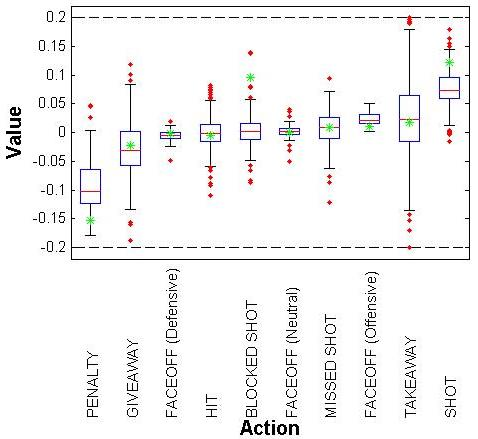
\includegraphics[width = 1.0\columnwidth]{boxplot_actionvalues4}
%\vspace{1in}
%\caption{Action Values}
%\label{fig:boxplot-action-values}
%\end{figure}

%[OS: use box plots]
%
%\begin{table}[htb]
%\caption{Lock and Schucker's Action Values (Previous Values) vs. Value Iteration Action Values}
%\label{table:action-values}
%\begin{center}
%\resizebox{1\columnwidth}{!}{
%\begin{tabular}{|c|c|c|c|c|c|}
%\hline
%\bf{Action} & \bf{Previous Value} & \multicolumn{4}{|c|}{\bf{Value Iteration}} \\ \cline{3-6}
% & & Weighted Average & Maximum & Minimum & Variance \\ \hline
%Blocked Shot & 0.0957 & 0.0004 & 0.5025 & -0.5785 & 0.0004 \\ \hline
%Faceoff (Defensive) & -0.0017 & & & & \\ \hline
%Faceoff (Neutral) & 0.0007 & & & & \\ \hline
%Faceoff (Offensive) & 0.0110 & & & & \\ \hline
%Giveaway & -0.0226 & -0.0020 & 0.5609 & -0.6065 & 0.0006 \\ \hline
%Hit & -0.0046 & -0.0001 & 0.6057 & -0.5208 & 0.0003 \\ \hline
%Missed Shot & 0.0094 & -0.0004 & 0.5890 & -0.6009 & \\ \hline
%Penalty & -0.1534 & -0.0072 & 0.1364 & -0.1920 & \\ \hline
%Shot & 0.1226 & 0.0063 & 0.5804 & -0.5008 & \\ \hline
%Takeaway & 0.0174 & 0.0018 & 0.5530 & -0.5763 & \\ \hline
%\end{tabular}
%}
%\end{center}
%\end{table}



\subsection{PLAYER VALUATIONS}
\label{subsec:player-valuations}

\begin{table}[htb]
\caption{2013-2014 Top-8 Player Impact Scores For Goals}
\label{table:top-player-impact-goals}
\begin{center}
\resizebox{1\columnwidth}{!}{
\begin{tabular}{|l|c|c|c|r|}
\hline
\bf{Name} & \bf{Goal Impact} & \bf{Points} & \bf{+/-} & \bf{Salary} \\ \hline
Jason Spezza & 29.64 & 66 & -26 & \$5,000,000 \\ \hline
Jonathan Toews & 28.75 & 67 & 25 & \$6,500,000 \\ \hline
Joe Pavelski & 27.20 & 79 & 23 & \$4,000,000 \\ \hline
Marian Hossa & 26.12 & 57 & 26 & \$7,900,000 \\ \hline
Patrick Sharp & 24.43 & 77 & 12 & \$6,500,000 \\ \hline
Sidney Crosby & 24.23 & 104 & 18 & \$12,000,000 \\ \hline
Claude Giroux & 23.89 & 86 & 7 & \$5,000,000 \\ \hline
Tyler Seguin & 23.89 & 84 & 16 & \$4,500,000 \\ \hline
%Max Pacioretty & 22.54 & 60 & 8 & \$4,000,000 \\ \hline
%Patrice Bergeron & 22.26 & 62 & 38 & \$4,550,000 \\ \hline
\end{tabular}
}
\end{center}
\end{table}

As players perform actions on behalf of their team, it is intuitive to apply the impact scores of team actions to the players performing the action, yielding player valuations.
To calculate player valuations, we apply the impact of an action to the player as they perform the action.
Next, we sum the impact scores of a player's actions over a single game, and then over a single season, to compute a net season impact score for the player. This procedure is equivalent to comparing the actions taken by a specific player to those of the league-average player, similar to previous work \citep{Pettigrew2015,Cervone2014a}.
We compare impact on Next Goal Scored with three other player ranking metrics: points earned, salary, and +/-.
To avoid confounding effects between different seasons, we use only the most recent full season, 2013-2014.
Player impact scores are shown in Table~\ref{table:top-player-impact-goals}. Tables for all seasons are available as well \citep{Routley2015}.
Figure~\ref{fig:points-vs-impact} shows that next goal impact correlates well with points earned. A point is earned for each goal or assist by a player.
%Players with high impact on goal tend to have high salaries as they help their team to produce more goals. However, the magnitude player salaries vary greatly regardless of the magnitude of their impact score, and the median salary is \$2.4 million USD.
%We observe in Figure~\ref{fig:scatterplot-salary-impact} that player salaries vary wildly regardless of their impact score, although salaries tend to increase as impact score increases.
Since these players have a high impact on goals, they also tend to have a positive +/- rating.
%Since +/- incorporates information about teammates on the ice, this indicates that our method captures enough information about individuals by analyzing an entire play sequence, rather than scoring a line as a whole. OS: I'm quite worried about this point, the best way is probably to compute scores both ways.
Jason Spezza is an anomaly, as he has the highest impact score but a very negative +/- score. This is due to his team performing poorly overall in the 2013-2014 season, and the team overall had a goal differential of -29, one of the highest goal differentials that season. This example shows that impact scores distinguish a player who generally performs useful actions but happens to be on a poor team.

In Table~\ref{table:top-player-impact-penalties}, we see player impact with respect to Next Penalty Received. High impact numbers indicate a tendency to cause penalties for a player's own team, or prevent penalties for the opponent. We compare the Q-function impact numbers to Penalties in Minutes (PIM), +/-, and salary. Players with high Q-function numbers have high penalty minutes as we would expect. They also have low +/-, which shows the importance of penalties for scoring chances. Their salaries tend to be lower. There are however notable exceptions, such as Dion Phaneuf, who draws a high salary although his actions have a strong tendency to incur penalties.

%\begin{figure}[ht]
%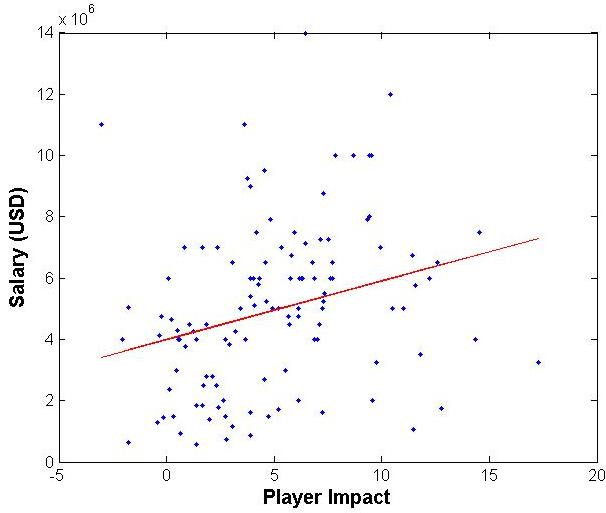
\includegraphics[width = 1.0\columnwidth]{player_impact_vs_salary}
%\vspace{1in}
%\caption{2014-2015 Salary Vs. Player Impact For Goals}
%\label{fig:scatterplot-salary-impact}
%\end{figure}

\begin{table}[htb]
\caption{2013-2014 Top-8 Player Impacts For Penalties}
\label{table:top-player-impact-penalties}
\begin{center}
\resizebox{1\columnwidth}{!}{
\begin{tabular}{|l|c|c|c|r|}
\hline
\bf{Name} & \bf{Penalty Impact} & \bf{PIM} & \bf{+/-} & \bf{Salary} \\ \hline
Chris Neil & 62.58 & 211 & -10 & \$2,100,000 \\ \hline
Antoine Roussel & 54.26 & 209 & -1 & \$625,000 \\ \hline
%Radko Gudas & 53.34 & 152 & 2 & \$575,000 \\ \hline
Dion Phaneuf & 52.52 & 144 & 2 & \$5,500,000 \\ \hline
Zac Rinaldo & 48.65 & 153 & -13 & \$750,000 \\ \hline
Rich Clune & 47.08 & 166 & -7 & \$525,000 \\ \hline
Tom Sestito & 46.34 & 213 & -14 & \$650,000 \\ \hline
%Tom Wilson & 46.12 & 151 & 1 & \$925,000 \\ \hline
Zack Smith & 44.55 & 111 & -9 & \$1,500,000 \\ \hline
David Perron & 42.49 & 90 & -16 & \$3,500,000 \\ \hline
\end{tabular}
}
\end{center}
\end{table}

\section{LESION STUDY}
We evaluate the components of our full model by considering simpler  models.

\subsection{USING AVERAGE ACTION VALUES}

We  compare context-aware action values vs. fixed action values (as in THoR) in terms of   the entropy of the Next Goal conditional probabilities. This quantifies the information lost by ignoring context.
Table~\ref{table:entropy} shows the average entropy for context-aware and context-unaware probabilities.
%
%For each action-state pair, the compute the entropy of the corresponding Next Goal probability.
%The average of these entropies is the action-state average.
The {\em context-unaware} Next Goal probability for an action event, is the marginal probability obtained from action-state probabilities by averaging over all states where the action is taken. For all action events, this marginal probability of Next Goal Away is between 47\% and 48\%.
This leads to an average context-unaware entropy of 0.9741 with standard deviation of only 0.0012.
The average of the context-aware entropies is 0.9582, which is a lower uncertainty than the context-unaware model; but  these entropies show considerable variance, ranging smoothly from 0 to 1, with a large standard deviation of 0.1482.
The large standard deviation demonstrates that including context in the model causes the predictive uncertainty of each state to vary more than a context-unaware model, however, it tends to create higher predictive accuracy with a lower average entropy.
The entropy results are statistically significant according to the paired t-test (p $=2.8\times10^{-8}$).

\begin{table}[htb]
\caption{Context-Aware vs. Context-Unaware Entropies.}
\label{table:entropy}
\begin{center}
\resizebox{1\columnwidth}{!}{
%\begin{tabular}{|r|r|r|r|}\hline
%\bf{Context-Aware Average} & \bf{Standard Dev.} & \bf{Context-Unaware Average} & \bf{Standard Dev.}\\
%0.9582 & 0.1482 & 0.9741 & 0.0012
\begin{tabular}{|l|r|r|r|}
\hline
\bf{Action} & \begin{tabular}{c} \bf{Context-Unaware} \\ \textbf{Probability}\\ \bf{Of Next Goal} \end{tabular}
& \begin{tabular}{c} \bf{Context-Unaware} \\ \textbf{Entropy} \end{tabular} & \begin{tabular}{c} \bf{Average} \\ \textbf{Context-Aware} \\ \textbf{Entropy} \end{tabular} \\ \hline
Blocked Shot & 0.4840 & 0.9993 & \bf{0.9455} \\ \hline
Faceoff (Defensive) & 0.4828 & 0.9991 & \bf{0.9913} \\ \hline
Faceoff (Neutral) & 0.5025 & 1.0000 & \bf{0.9944} \\ \hline
Faceoff (Offensive) & 0.5335 & 0.9968 & \bf{0.9876} \\ \hline
Giveaway & 0.4907 & 0.9997 & \bf{0.9271} \\ \hline
Hit & 0.4985 & 1.0000 & \bf{0.9462} \\ \hline
Missed Shot & 0.5178 & 0.9991 & \bf{0.9413} \\ \hline
Penalty & 0.4442 & 0.9910 & \bf{0.9833} \\ \hline
Shot & 0.5673 & 0.9869 & \bf{0.8951} \\ \hline
Takeaway & 0.5125 & 0.9995 & \bf{0.9279} \\ \hline
\hline
\multicolumn{2}{|c|}{Average Entropy Over Actions} & 0.9971 & \bf{0.9540} \\ \hline
\end{tabular}
}
\end{center}
\end{table}



\subsection{EXAMINING PROPAGATION EFFECTS}
\label{subsec:lesion-study}


The transition graph construction algorithm facilitates changing the possible state transitions. We utilize this in our experiments to study how different propagation models affect the impact of actions on Next Goal Scored. Specifically, we consider three different transitions graphs of increasing density, their sizes shown in Table~\ref{table:size-of-graphs}. The number of states/nodes 1,325,809 is the same for all graphs.

\begin{description}
\item[Local Transitions Only]  State transitions occur only within a play sequence, not across play sequences.
\item[Penalty Transitions] State transitions occur from penalty leaf nodes to successor context nodes.
\item[Full Transition Graph] Includes loopback edges from all leaf nodes to context nodes, as defined in Section~\ref{subsec:play-sequences}.
\end{description}

\begin{table}[htb]
\caption{Size of State Transition Graphs}
\label{table:size-of-graphs}
\begin{center}
\resizebox{\columnwidth}{!}{
\begin{tabular}{|l|c|c|c|}
\hline
& \bf{Local} & \bf{Penalty} & \bf{Full} \\ \hline
%\bf{Number of Nodes} & 1,325,809 & 1,325,809 & 1,325,809 \\ \hline
\bf{Number of Edges} & 1,325,808 & 1,382,780 & 1,662,504 \\ \hline
\end{tabular}
}
\end{center}
\end{table}


%Three different state transition graphs were used in our experiments as outlined in Section~\ref{subsec:mdp-construction}.
Action impact changes value depending on the state transition graph. The average differences in action values of the same states across different transition graphs, as well as the standard deviation of the differences, are shown in Table~\ref{table:change-in-action-values}. The table shows that the impact on who scores the next goal changes as more information is propagated between states.


{\em Penalty vs. Local.}
With the local transition graph, value iteration computes the impact of an action on the current play sequence only.
Thus the Q-value differential for context states, with the initial empty play sequence, can be obtained from Table~\ref{table:context-statistics}.
The penalty transition graph propagates to the next sequence the effect of penalties only. This means that if a play sequence ends with an event other than a penalty or goal (e.g., stoppage) the penalty transition model treats the play as ending with that event. Thus there is no propagation of the effect of a penalty. In hockey terms, with the local transition graph, the model is not aware that a penalty is followed by a powerplay.
Propagating the effect of penalties changes most the estimation of the impact of penalties.
This change reflects that receiving a penalty lowers the chances of scoring the next goal.
Less obviously, winning a faceoff in the offensive zone has a relatively high positive indirect impact on scoring the next goal, via increasing the probability of a penalty against the opposing team.
The effect of winning an offensive zone faceoff can also be seen in Figure~\ref{fig:penalty-impact}.

{\em Full vs. Penalty.} In hockey terms, with the penalty transition graph, the model is aware that a penalty is followed by a {\em single} powerplay sequence. But if more than one sequence occurs in the same powerplay, the second sequence is ignored in the lookahead. The full transition graph propagates the information about the manpower advantage, until the context features are updated when the dynamics reaches a new context state.
Comparing the full transition graph with penalty propagation only, we still find the strongest average impact change for penalties. The simplest explanation of this result is that often in hockey, the effect of penalties goes beyond a single play sequence, and the full transition graph captures more of this medium-term effect.
%This shows that penalties have ripple effects on goals via events other than penalties.
%Scoring a goal also has a long-term effect of increasing the change of a penalty, as shown in Figure~\ref{fig:penalty-impact}.
%This indirect impact is shared by Offensive Zone Faceoff Wins. %, via their impact on Penalties.

While the aggregate differential effects show that more propagation leads to more informative results, they do not reflect the considerable context dependence shown by the standard deviations of the impact differentials.

\begin{table}[htb]
\caption{Action Impact {\em Differences} For The Next Goal Depending on Propagation Model.}
\label{table:change-in-action-values}
\begin{center}
\resizebox{1\columnwidth}{!}{
\begin{tabular}{|l|r|r|r|r|}
\hline
& \multicolumn{2}{|c|}{\bf{Full vs. Penalty}} & \multicolumn{2}{|c|}{\bf{Penalty vs. Local}} \\ \cline{2-5}
\bf{Action} & \bf{Average} & \bf{Std. Dev.} & \bf{Average} & \bf{Std. Dev.}\\ \hline
Blocked Shot & 0.0001 & 0.0210 & -0.0003 & 0.0126 \\ \hline
Faceoff (Defensive) & -0.0030 & 0.0455 & -0.0018 & 0.0225 \\ \hline
Faceoff (Neutral) & 0.0013 & 0.0464 & 0.0006 & 0.0203 \\ \hline
Faceoff (Offensive) & 0.0038 & 0.0432 & 0.0024 & 0.0260 \\ \hline
Giveaway & -0.0003 & 0.0245 & -0.0001 & 0.0142 \\ \hline
Hit & 0.0000 & 0.0194 & -0.0001 & 0.0126 \\ \hline
Missed Shot & -0.0001 & 0.0218 & 0.0003 & 0.0130 \\ \hline
Penalty & \bf{-0.0190} & 0.0278 & \bf{-0.0235} & 0.0337 \\ \hline
Shot & 0.0002 & 0.0191 & 0.0002 & 0.0103 \\ \hline
Takeaway & 0.0006 & 0.0245 & 0.0003 & 0.0146 \\ \hline
\end{tabular}
}
\end{center}
\end{table}

%\begin{table}[htb]
%\caption{Difference In Action Impact Values for Next Goal Scored, for different transition graphs.}
%\label{table:change-in-action-values}
%\begin{center}
%\resizebox{1\columnwidth}{!}{
%\begin{tabular}{|l|r|r|r|r|}
%\hline
%\bf{Action} & \bf{Full - Local} & \bf{Full - Penalty} & \bf{Penalty - Local} \\ \hline
%Blocked Shot & -0.0002 & 0.0001 & -0.0003 \\ \hline
%Faceoff (Defensive) & -0.0048 & -0.0030 & -0.0018 \\ \hline
%Faceoff (Neutral) & 0.0018 & 0.0013 & 0.0006 \\ \hline
%Faceoff (Offensive) & 0.0062 & 0.0038 & 0.0024 \\ \hline
%Giveaway & -0.0004 & -0.0003 & -0.0001 \\ \hline
%Hit & 0.0000 & 0.0000 & -0.0001 \\ \hline
%Missed Shot & 0.0002 & -0.0001 & 0.0003 \\ \hline
%Penalty & -0.0425 & -0.0190 & -0.0235 \\ \hline
%Shot & 0.0005 & 0.0002 & 0.0002 \\ \hline
%Takeaway & 0.0008 & 0.0006 & 0.0003 \\ \hline
% & \multicolumn{2}{|c|}{\bf{Full vs. Local}} & \multicolumn{2}{|c|}{\bf{Full vs. Penalty}} \\ \hline
%\bf{Action} & \bf{Average} & \bf{Std. Dev.} & \bf{Average} & \bf{Std. Dev.}\\ \hline
%Blocked Shot & -0.0002 & 0.0386 & 0.0001 & 0.0210 \\ \hline
%Faceoff (Defensive) & -0.0048 & 0.0554 & -0.0030 & 0.0455 \\ \hline
%Faceoff (Neutral) & 0.0018 & 0.0538 & 0.0013 & 0.0464 \\ \hline
%Faceoff (Offensive) & {\em 0.0062} & 0.0555 & {\em 0.0038} & 0.0432 \\ \hline
%Giveaway & -0.0004 & 0.0331 & -0.0003 & 0.0245 \\ \hline
%Hit & 0.0000 & 0.0279 & 0.0000 & 0.0194 \\ \hline
%Missed Shot & 0.0002 & 0.0297 & -0.0001 & 0.0218 \\ \hline
%Penalty & \bf{-0.0425} & 0.0609 & \bf{-0.0190} & 0.0278 \\ \hline
%Shot & 0.0005 & 0.0248 & 0.0002 & 0.0191 \\ \hline
%Takeaway & 0.0008 & 0.0333 & 0.0006 & 0.0245 \\ \hline
%\end{tabular}
%}
%\end{center}
%\end{table}

%\paragraph{Entropy Difference.} Maybe it's too complicated doing this for the three graphs. Apples to apples: i) local transition graph vs. context states only (Table~\ref{table:context-statistics}). ii) Base Entropy vs. context state entropy vs. full propagation. Or maybe iii) for each action, aggregate prob of next goal over all states, weighting by frequency of state. Then compare the resulting entropy for each action to average entropy over all states, weighting each state-action entropy by frequency of state.

%The entropy of the three state transition graphs is shown in Table~\ref{table:model-entropy}. The entropy of the Markov Game Model is lowest in the full model containing all loopback edges, showing that the full model is a more informative model. The entropy is still close to 1, as the probability of goal scoring is approximately even, with a slight home team advantage, as shown in Table~\ref{table:context-statistics}.

%
%\begin{table}[htb]
%\caption{Model Entropy}
%\label{table:model-entropy}
%\begin{center}
%\resizebox{1\columnwidth}{!}{
%\begin{tabular}{|l|c|c|}
%\hline
%\bf{Model} & \bf{Entropy} & \bf{Change In Entropy From Local} \\ \hline
%Local & 0.99816 & N/A \\ \hline
%Penalty & 0.99795 & -0.00021 \\ \hline
%Full & 0.99789 & -0.00027 \\ \hline
%\end{tabular}
%}
%\end{center}
%\end{table}


%\subsection{VALUE ITERATION}
%
%\subsection{REWARD FUNCTION = WIN}
%
%Back up wins. Show that after conditioning, agrees with observed frequency. [maybe other interesting states as well.]

%\subsection{REWARD FUNCTION = GOAL}
%
%Back up computes expected goals. How to evaluate?
%
%\subsection{REWARD FUNCTION = NEXT GOAL}
%
%When a goal is scored, finish process. Interpretation: probability that next goal is scored by team. Evaluate using a separate tree for data counts.

%\section{APPLICATIONS}



%\subsection{HYPOTHESES}

%A nice way to structure this section and to engage the referees is to give a list of what you want to establish through your experiments, before you give the details of your experiments. This usually also clarifies things for yourself. Hopefully you have more interesting hypotheses to test than ``I can find some datasets on which the predictive accuracy of my system is higher than that of some previous methods.''

%Describe briefly your set-up, e.g. RAM, Processor, programming language.

%\subsection{DATASETS}



%\begin{table}[htb]
%\caption{Size of Markov Decision Process Graph}
%\label{table:size-of-mdp}
%\begin{center}
%\resizebox{\columnwidth}{!}{
%\begin{tabular}{|l|c|c|c|}
%\hline
%& \bf{No Manpower Differential} & \bf{With Manpower Differential} \\ \hline
%\bf{Number of Nodes} & 1,208,623 & 1,325,813 \\ \hline
%\bf{Number of Edges} & 1,508,247 & 1,662,509 \\ \hline
%\end{tabular}
%}
%\end{center}
%\end{table}

%Outline the datasets that you are using. Highlight interesting aspects. Give summary statistics (e.g., data set sizes). Are they real-world or synthetic?

%It can be a good idea to present your data in terms of sample training and test sets.

%\subsection{METHODS COMPARED}

%List all of the methods. Make sure you explain which methods are yours and which were proposed by other researchers. Explain settings of methods, and why you chose them.

%\subsection{PERFORMANCE MEASURES}

%Explain what you are measuring (e.g., runtime, accuracy) etc. More is better. How are you computing the numbers? E.g., with cross-validation, taking averages? Usually referees like you to add error bars or standard deviations.

%\subsection{RESULTS}

%You need to report results for triples of (method, datasets, metric). This kind of three-dimensional setting is not easy to translate into graphs but you should try. It's best to try and find graphs that support your points; refer back to the hypotheses listed above. I suggest importing  your data into a spreadsheet program, which allows you to produce many charts. Also, there are macros that convert Excel tables into latex tables. This saves you a lot of the pain of producing Latex tables. Avoid color graphs because referees may be printing on black and white, and in any case the conference proceedings won't be in color.

\section{CONCLUSION}

%[Propagating action effects across sequences utilizes the ordering play sequences in a game, rather than treating sequences as an unordered independent set.]
%[We leverage this computational capability to propagate the impact of an action on reward events like goals and penalties that may occur after the action was taken. These effects are propagated along a sequence and even across sequences.]
%[Another difference is previous models focus on goals and use a Poisson model to estimate scoring rates in continuous time. We use a discrete-time model as is common in machine learning, and leave a continuous time hockey Markov model for future work.]
We have constructed a Markov Game Model for a massive set of NHL play-by-play events with a rich state space.% that utilizes much of the information in the data.
Tree-based data structures support efficient parameter estimation and storage. Value iteration computes the values of each action given its context and sequence history---the Q-function of the model. Compared to previous work that assigns a single value to actions, the Q-function incorporates two powerful sources of information for valuing hockey actions: (1) It takes into account the context of the action, represented by the Markov Game state. (2) It models the medium-term impact of an action by propagating its effect to future states. %The Q-function provides knowledge about hockey dynamics by quantifying how much which action matters when.
Propagating action effects across sequences utilizes the ordering play sequences in a game, rather than treating sequences as an unordered independent set.
%
Analysis of the computed Q-function shows the impact of an action varies greatly with context, and medium-term ripple effects make a difference. We apply our model to evaluate the performance of players in terms of their actions' total impact. Action impact scores are calculated for players with respect to different objective functions. Impact scores for the next goal correlate with points and +/- statistics. The impact of players on the next penalty has to our knowledge
not been previously considered, and shows some surprises, as some highly-paid players hurt their team by causing penalties. %Another potential application for context-aware performance evaluation is in finding strengths and weaknesses of teams: We can use the Q-function to find situations in which a teams mix of actions provides a substantially different expected result from a generic team.
In sum, the Q-function is a powerful AI concept that captures much information about hockey dynamics as the game is played in the NHL.

\paragraph{Future Work} The NHL data provides a rich dataset for real-world event modelling. A number of further AI techniques can be applied to utilize even more of the available information than our Markov Game model does. A promising direction is to extend our Markov Game model, which is discrete with data about continuous quantities. These include (i) the time between events, %---which requires a continuous time Markov Game model,
(ii) the absolute game time of the events, % (e.g. ``minute 15''),
(iii) location of shots \citep{Krzywicki2005}.
% (however, reported shot locations are noisy ). % Player locations would be valuable information, but are currently not available for actions other than shots.
%
Our use of reinforcement learning techniques has been mainly for finding patterns in a rich data set, in the spirit of descriptive statistics and data mining. Another goal is to {\em predict} a player or team's future performance based on past performance using machine learning techniques. %For example, can we predict a player's performance in the next season based on the previous seasons?
%Machine learning methods aim to provide reliable generalization, and can be combined with dynamic programming for predicting future performance \citep{bib:sutton}.
For example, sequence modelling would be able to generalize from play sequence information. A promising model class are Piecewise Constant Conditional Intensity Models for continuous time event sequences \citep{Gunawardana2011,Parikh2012}. These models are especially well suited for sequences with a large set of possible events, such as our action events. Another extension is to evaluate players with respect to similar players \citep{Cervone2014a}, for instance players who play the same position.

A potential future application for improving play and advising coaches is in finding strengths and weaknesses of teams: We can use the Q-function to find situations in which a team's mix of actions provides a substantially different expected result from that of a generic team.
We leave this application for future work.

\section*{Acknowledgements} This work was supported by a Discovery Grant from the National Sciences and Engineering Council of Canada. We received helpful comments from Tim Swartz and anonymous UAI referees. Zeyu Zhang assisted with the preparation of plots.

%[Kurt: should we insert your preliminary results]
%
%descriptive vs. predictive
%
%Finding an efficient way to model the available temporal play sequence duration, such as in \citep{Parikh2012}, and player shift change data alongside the Markov Game Model would be an interesting study, and could be used to form simulations of NHL games. Goalies do not participate in many recorded events, so it is difficult to evaluate goalies with this model, and extension methods for evaluating goaltenders are left as future work. Learning what context features and action features, such as shot location and shot type \citep{Krzywicki2005}, perform better than others could also be an interesting study.

%This should be a summary of the main points and what your findings were. Repeat why these results are significant. Often it's a good idea to add some avenues for future work. Often reviewers think ``yes, but you should also have done xyz''. If you can guess what xyz is, you can mention it as an avenue for future work, and then you have shown that you did think of xyz and you acknowledge its importance.

%\section{REFERENCES} Students don't pay nearly enough attention to references. Referees get turned off if the references are incomplete, hard to read, etc., especially if this is is the case for citations to their own work.

%\section{FIRST LEVEL HEADINGS}
%
%First level headings are all caps, flush left, bold and in point size
%12. One line space before the first level heading and 1/2~line space
%after the first level heading.
%
%\subsection{SECOND LEVEL HEADING}
%
%Second level headings must be flush left, all caps, bold and in point
%size 10. One line space before the second level heading and 1/2~line
%space after the second level heading.
%
%\subsubsection{Third Level Heading}
%
%Third level headings must be flush left, initial caps, bold, and in
%point size 10.  One line space before the third level heading and
%1/2~line space after the third level heading.
%
%\vskip .5pc
%Fourth Level Heading
%
%Fourth level headings must be flush left and initial caps.
%One line space before the fourth level heading and 1/2~line space
%after the fourth level heading.

%\subsection{CITATIONS, FIGURES, REFERENCES}


%\subsubsection{Citations in Text}
%
%Citations within the text should include the author's last name and
%year, e.g., (Cheesman, 1985). Reference style should follow the style
%that you are used to using, as long as the citation style is
%consistent.
%
%For the original submission, take care not to reveal the authors' identity through
%the manner in which one's own previous work is cited.  For example, writing
%``In (Bovik, 1970), we studied the problem of AI'' would be inappropriate, as
%it reveals the author's identity.  Instead, write ``(Bovik, 1970) studied the
%problem of AI.''

%\subsubsection{Footnotes}
%
%Indicate footnotes with a number\footnote{Sample of the first
%footnote} in the text. Use 8 point type for footnotes.  Place the
%footnotes at the bottom of the page on which they appear.  Precede the
%footnote with a 0.5 point horizontal rule 1~inch (6~picas)
%long.\footnote{Sample of the second footnote}

%\subsubsection{Figures}
%
%All artwork must be centered, neat, clean, and legible. Figure number
%and caption always appear below the figure.  Leave 2 line spaces
%between the figure and the caption. The figure caption is initial caps
%and each figure numbered consecutively.
%
%Make sure that the figure caption does not get separated from the
%figure. Leave extra white space at the bottom of the page rather than
%splitting the figure and figure caption.
%\begin{figure}[ht]
%\vspace{1in}
%\caption{Sample Figure Caption}
%\end{figure}

%\subsubsection{Tables}
%
%All tables must be centered, neat, clean, and legible. Table number
%and title always appear above the table.  %See
%Table~\ref{sample-table}.
%
%One line space before the table title, one line space after the table
%title, and one line space after the table. The table title must be
%initial caps and each table numbered consecutively.
%
%\begin{table}[h]
%\caption{Sample Table Title}
%\label{sample-table}
%\begin{center}
%\begin{tabular}{ll}
%\multicolumn{1}{c}{\bf PART}  &\multicolumn{1}{c}{\bf DESCRIPTION} \\
%\hline \\
%Dendrite         &Input terminal \\
%Axon             &Output terminal \\
%Soma             &Cell body (contains cell nucleus) \\
%\end{tabular}
%\end{center}
%\end{table}

\newpage

%\subsubsection*{Acknowledgements}

%Use unnumbered third level headings for the acknowledgements title.
%All acknowledgements go at the end of the paper.


%\subsubsection*{References}

%References follow the acknowledgements.  Use unnumbered third level
%heading for the references title.  Any choice of citation style is
%acceptable as long as you are consistent.

%NOTE: NEED TO USE CORRECT REFERENCES HEADER
\bibliographystyle{apalike}
\renewcommand\bibsection{\subsubsection*{\refname}}
\bibliography{master}


%J.~Alspector, B.~Gupta, and R.~B.~Allen  (1989). Performance of a
%stochastic learning microchip.  In D. S. Touretzky (ed.), {\it Advances
%in Neural Information Processing Systems 1}, 748-760.  San Mateo, Calif.:
%Morgan Kaufmann.

%F.~Rosenblatt (1962). {\it Principles of Neurodynamics.} Washington,
%D.C.: Spartan Books.

%G.~Tesauro (1989). Neurogammon wins computer Olympiad.  {\it Neural
%Computation} {\bf 1}(3):321-323.

\end{document}
